\documentclass[11pt]{article}

\usepackage[final]{acl}
\usepackage{times}
\usepackage{latexsym}
\usepackage{multirow}
\usepackage[T1]{fontenc}
\usepackage[utf8]{inputenc}
\usepackage{microtype}

\usepackage{inconsolata}

\usepackage{amsmath}
\usepackage{amssymb}
\usepackage{mathtools}
\usepackage{amsthm}
\usepackage[capitalize,noabbrev]{cleveref}
\usepackage{threeparttable}
\usepackage[table]{xcolor} 
\usepackage{multirow} 
\usepackage{array} 
\usepackage{makecell}
\usepackage{booktabs}
\usepackage{xspace}

\usepackage{xcolor}
\usepackage{tcolorbox}
\tcbuselibrary{skins,breakable}
\usepackage{tikz}
\usepackage{fontawesome5}
\usepackage{booktabs}
\usepackage{titletoc}
\definecolor{headerblue}{RGB}{41, 128, 185}
\definecolor{metricgreen}{RGB}{39, 174, 96}
\definecolor{alertred}{RGB}{192, 57, 43}
\definecolor{warningyellow}{RGB}{243, 156, 18}
\definecolor{lightgray}{RGB}{245, 245, 245}
\definecolor{darkgray}{RGB}{52, 73, 94}
\definecolor{mutationpurple}{RGB}{142, 68, 173}
\definecolor{crossoverblue}{RGB}{52, 152, 219}



\newcommand{\method}{QuantaAlpha\xspace}


\title{\raisebox{-0.7em}{
\includegraphics[height=2em]{images/icon.jpg}} QuantaAlpha: An Evolutionary Framework for LLM-Driven \\ Alpha Mining}

% \vspace{20mm}

\author{
\textbf{Jun Han\textsuperscript{1*}},
 \textbf{Shuo Zhang\textsuperscript{2*}},
 \textbf{Wei Li\textsuperscript{1*}},
 \textbf{Zhi Yang\textsuperscript{1*}},
 \textbf{Yifan Dong\textsuperscript{1}},
 \textbf{Tu Hu\textsuperscript{2}},\\
 \textbf{Jialuo Yuan\textsuperscript{3}},
 \textbf{Xiaomin Yu\textsuperscript{2}},
 \textbf{Yumo Zhu\textsuperscript{1}},
 \textbf{Fangqi Lou\textsuperscript{1}},
 \textbf{Xin Guo\textsuperscript{1}},
 \textbf{Zhaowei Liu\textsuperscript{1}},\\
 \textbf{Tianyi Jiang\textsuperscript{4}},
 \textbf{Ruichuan An\textsuperscript{4}},
 \textbf{Jingping Liu\textsuperscript{5}},
 \textbf{Biao Wu\textsuperscript{2}},
 \textbf{Rongze Chen\textsuperscript{2}},
 \textbf{Kunyi Wang\textsuperscript{2}},\\  
 \textbf{Yifan Wang\textsuperscript{2}},
 \textbf{Sen Hu\textsuperscript{2,4}},
 \textbf{Xinbing Kong\textsuperscript{6\dag}},
 % \textbf{Liwen Zhang\textsuperscript{1\dag}},
 \textbf{Ronghao Chen\textsuperscript{2,4\dag}},
 \textbf{Huacan Wang\textsuperscript{2\dag}}
\\
\\
 \textsuperscript{1}SUFE\thanks{AIFin Lab: \href{mailto:aifinlab.sufe@gmail.com}{aifinlab.sufe@gmail.com}},
\textsuperscript{2}QuantaAlpha\thanks{QuantaAlpha: \href{mailto:quantaalpha.ai@gmail.com}{quantaalpha.ai@gmail.com}},
 \textsuperscript{3}Stanford,
  \textsuperscript{4}PKU,
  \textsuperscript{5}SYSU,
    \textsuperscript{6}SEU
    \vspace{2mm}
\\
\small {
    \textbf{{*}These authors contributed equally to this work.}
}
\\
 \small{
   \textbf{\dag Correspondence:} 
   \href{mailto:xinbingkong@126.com}{xinbingkong@126.com},
   % \href{mailto:zhang.liwen@shufe.edu.cn}{zhang.liwen@shufe.edu.cn},
\href{mailto:chenronghao@alumni.pku.edu.cn}{chenronghao@alumni.pku.edu.cn},
\href{mailto:wanghuacan17@mails.ucas.ac.cn}{wanghuacan17@mails.ucas.ac.cn}
 }
}

\makeatletter
\def\@fnsymbol#1{%
  \ifcase#1\or
    \ensuremath{\mathsection} % 1 -> §
  \or
    \ensuremath{\P}      % 2 -> †
  \or
    \ensuremath{\dagger}     % 3 -> ‡
  \or
    \ensuremath{\star}        % 4 -> *
  \else
    \@ctrerr
  \fi
}
\makeatother
\begin{document}
\maketitle
\begin{center}
    \vspace{20pt}
    \large
    \faGithub\hspace{6pt}\href{https://github.com/QuantaAlpha/QuantaAlpha}{\texttt{\color{black}https://github.com/QuantaAlpha/QuantaAlpha}}
\end{center}


\begin{abstract}
Financial markets are noisy and non-stationary, making alpha mining highly sensitive to noise in backtesting results and sudden market regime shifts. While recent agentic frameworks improve alpha mining automation, they often lack controllable multi-round search and reliable reuse of validated experience. To address these challenges, we propose \textbf{QuantaAlpha}, an evolutionary alpha mining framework that treats each end-to-end mining run as a trajectory and improves factors through trajectory-level mutation and crossover operations. QuantaAlpha localizes suboptimal steps in each trajectory for targeted revision and recombines complementary high-reward segments to reuse effective patterns, enabling structured exploration and refinement across mining iterations.
During factor generation, QuantaAlpha enforces semantic consistency across the hypothesis, factor expression, and executable code, while constraining the complexity and redundancy of the generated factor to mitigate crowding. Extensive experiments on the China Securities Index 300 (CSI 300) demonstrate consistent gains over strong baseline models and prior agentic systems. When utilizing GPT-5.2, QuantaAlpha achieves an Information Coefficient (IC) of 0.1501, with an Annualized Rate of Return (ARR) of 27.75\% and a Maximum Drawdown (MDD) of 7.98\%. Moreover, factors mined on CSI 300 transfer effectively to the China Securities Index 500 (CSI 500) and the Standard \& Poor's 500 Index (S\&P 500), delivering 160\% and 137\% cumulative excess return over four years, respectively, which indicates strong robustness of QuantaAlpha under market distribution shifts.
\end{abstract}

\begin{figure}[ht]
\centering
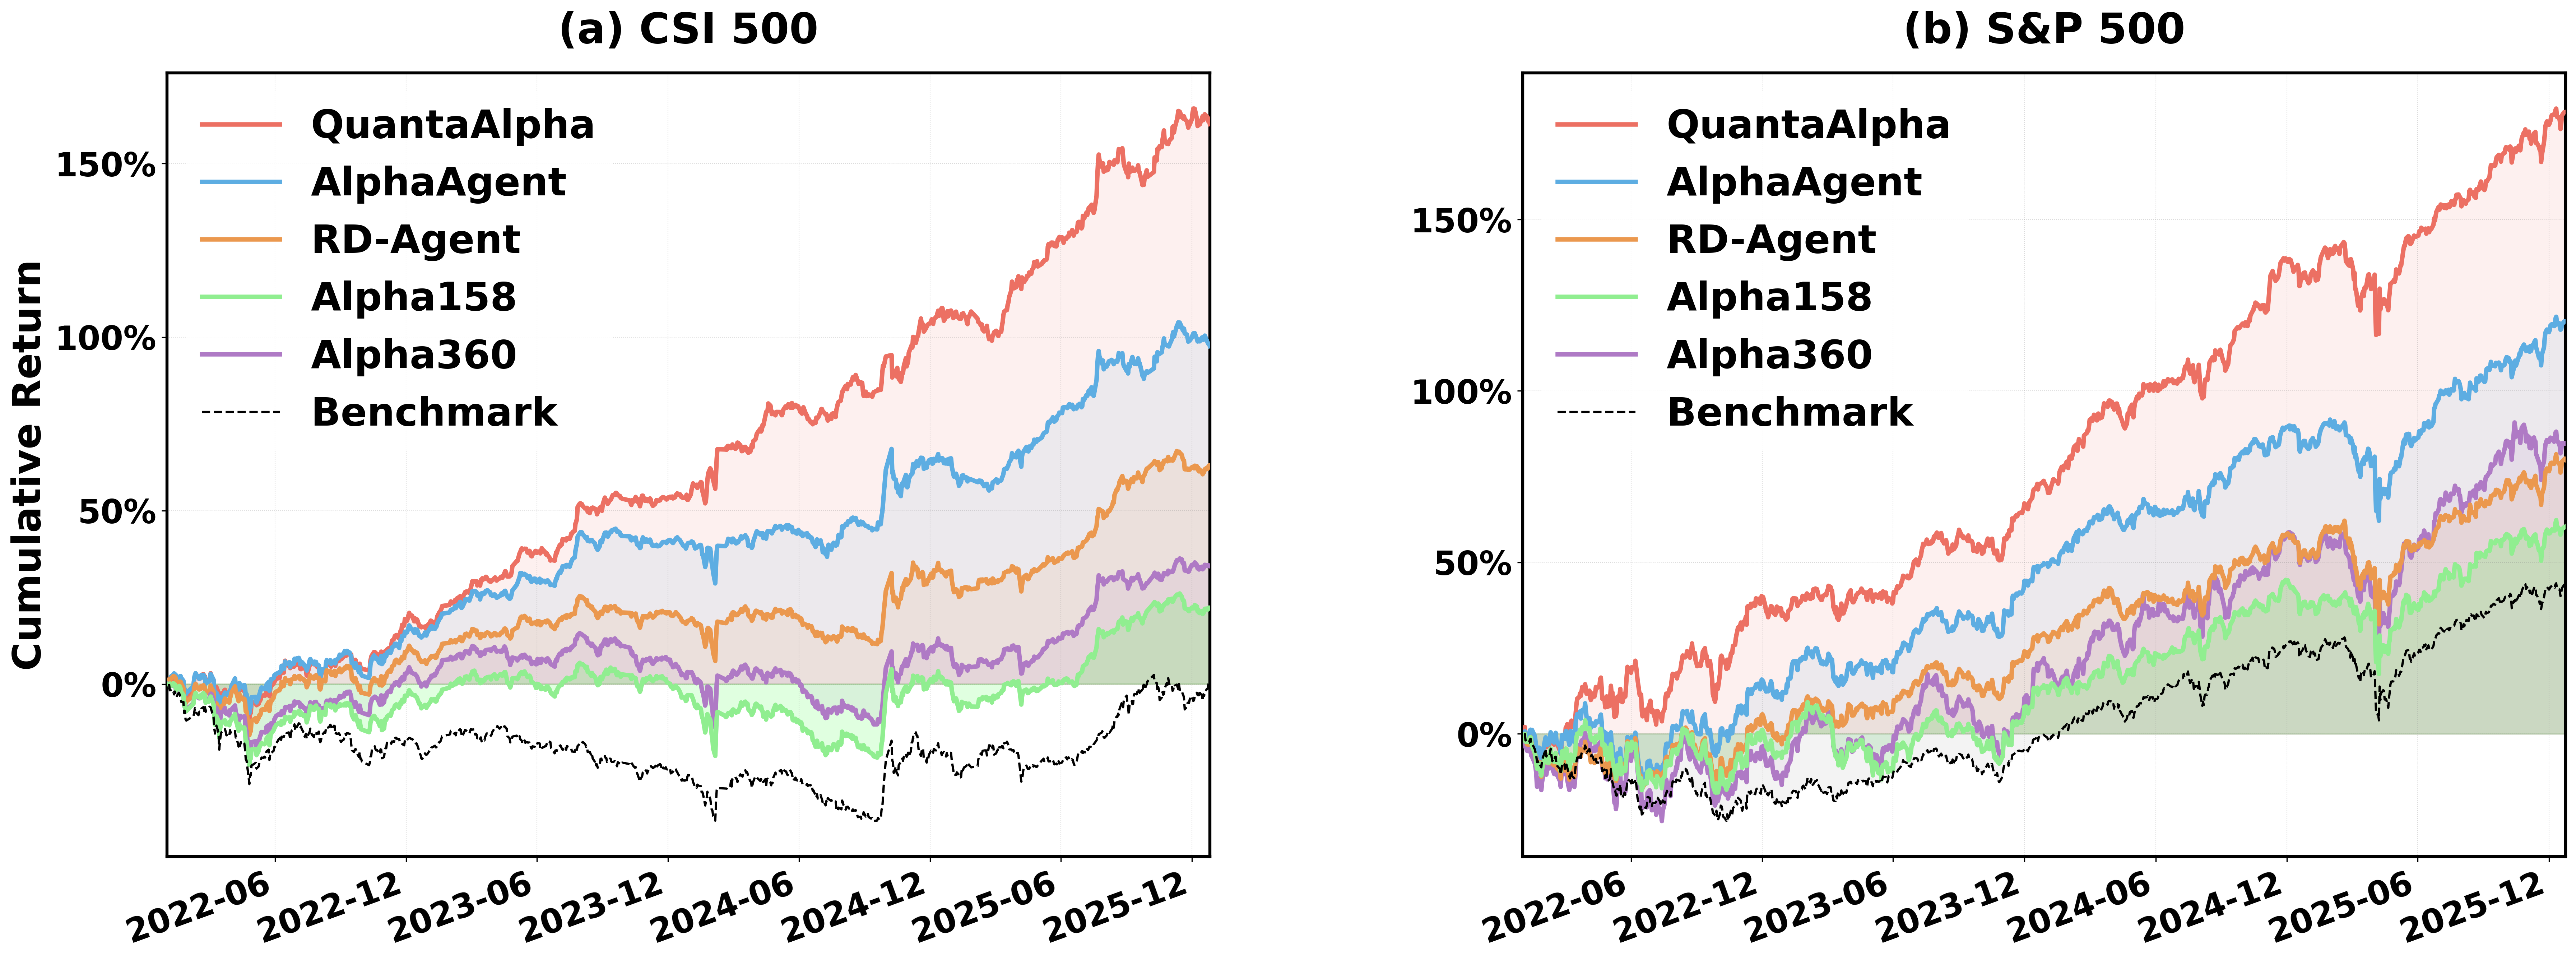
\includegraphics[width=0.78\textwidth]{images/figure3.png}
\caption{Cumulative excess returns of different approaches on CSI 500 and S\&P 500.}
\label{fig:cumulative_returns}
\end{figure}



\newpage



\section{Introduction}
Financial markets are high-dimensional, non-stationary stochastic systems, where returns exhibit heavy tails \cite{fama1965behavior}, time-varying volatility \cite{engle1982autoregressive}, and cross-sectional dependence \cite{pesaran2021general}. Quantitative investment therefore relies on alpha mining to extract predictive signals from noisy observations. Recently, large language models (LLMs) \cite{lope2025chatgpt} and LLM-based agent frameworks \cite{zhang2024multi, xiao2025trad} have been introduced into the factor research workflow. By leveraging advanced reasoning and code generation capabilities, these systems can automate factor construction and iteratively refine candidates through backtesting feedback.

\begin{figure}[htbp]
    \centering
    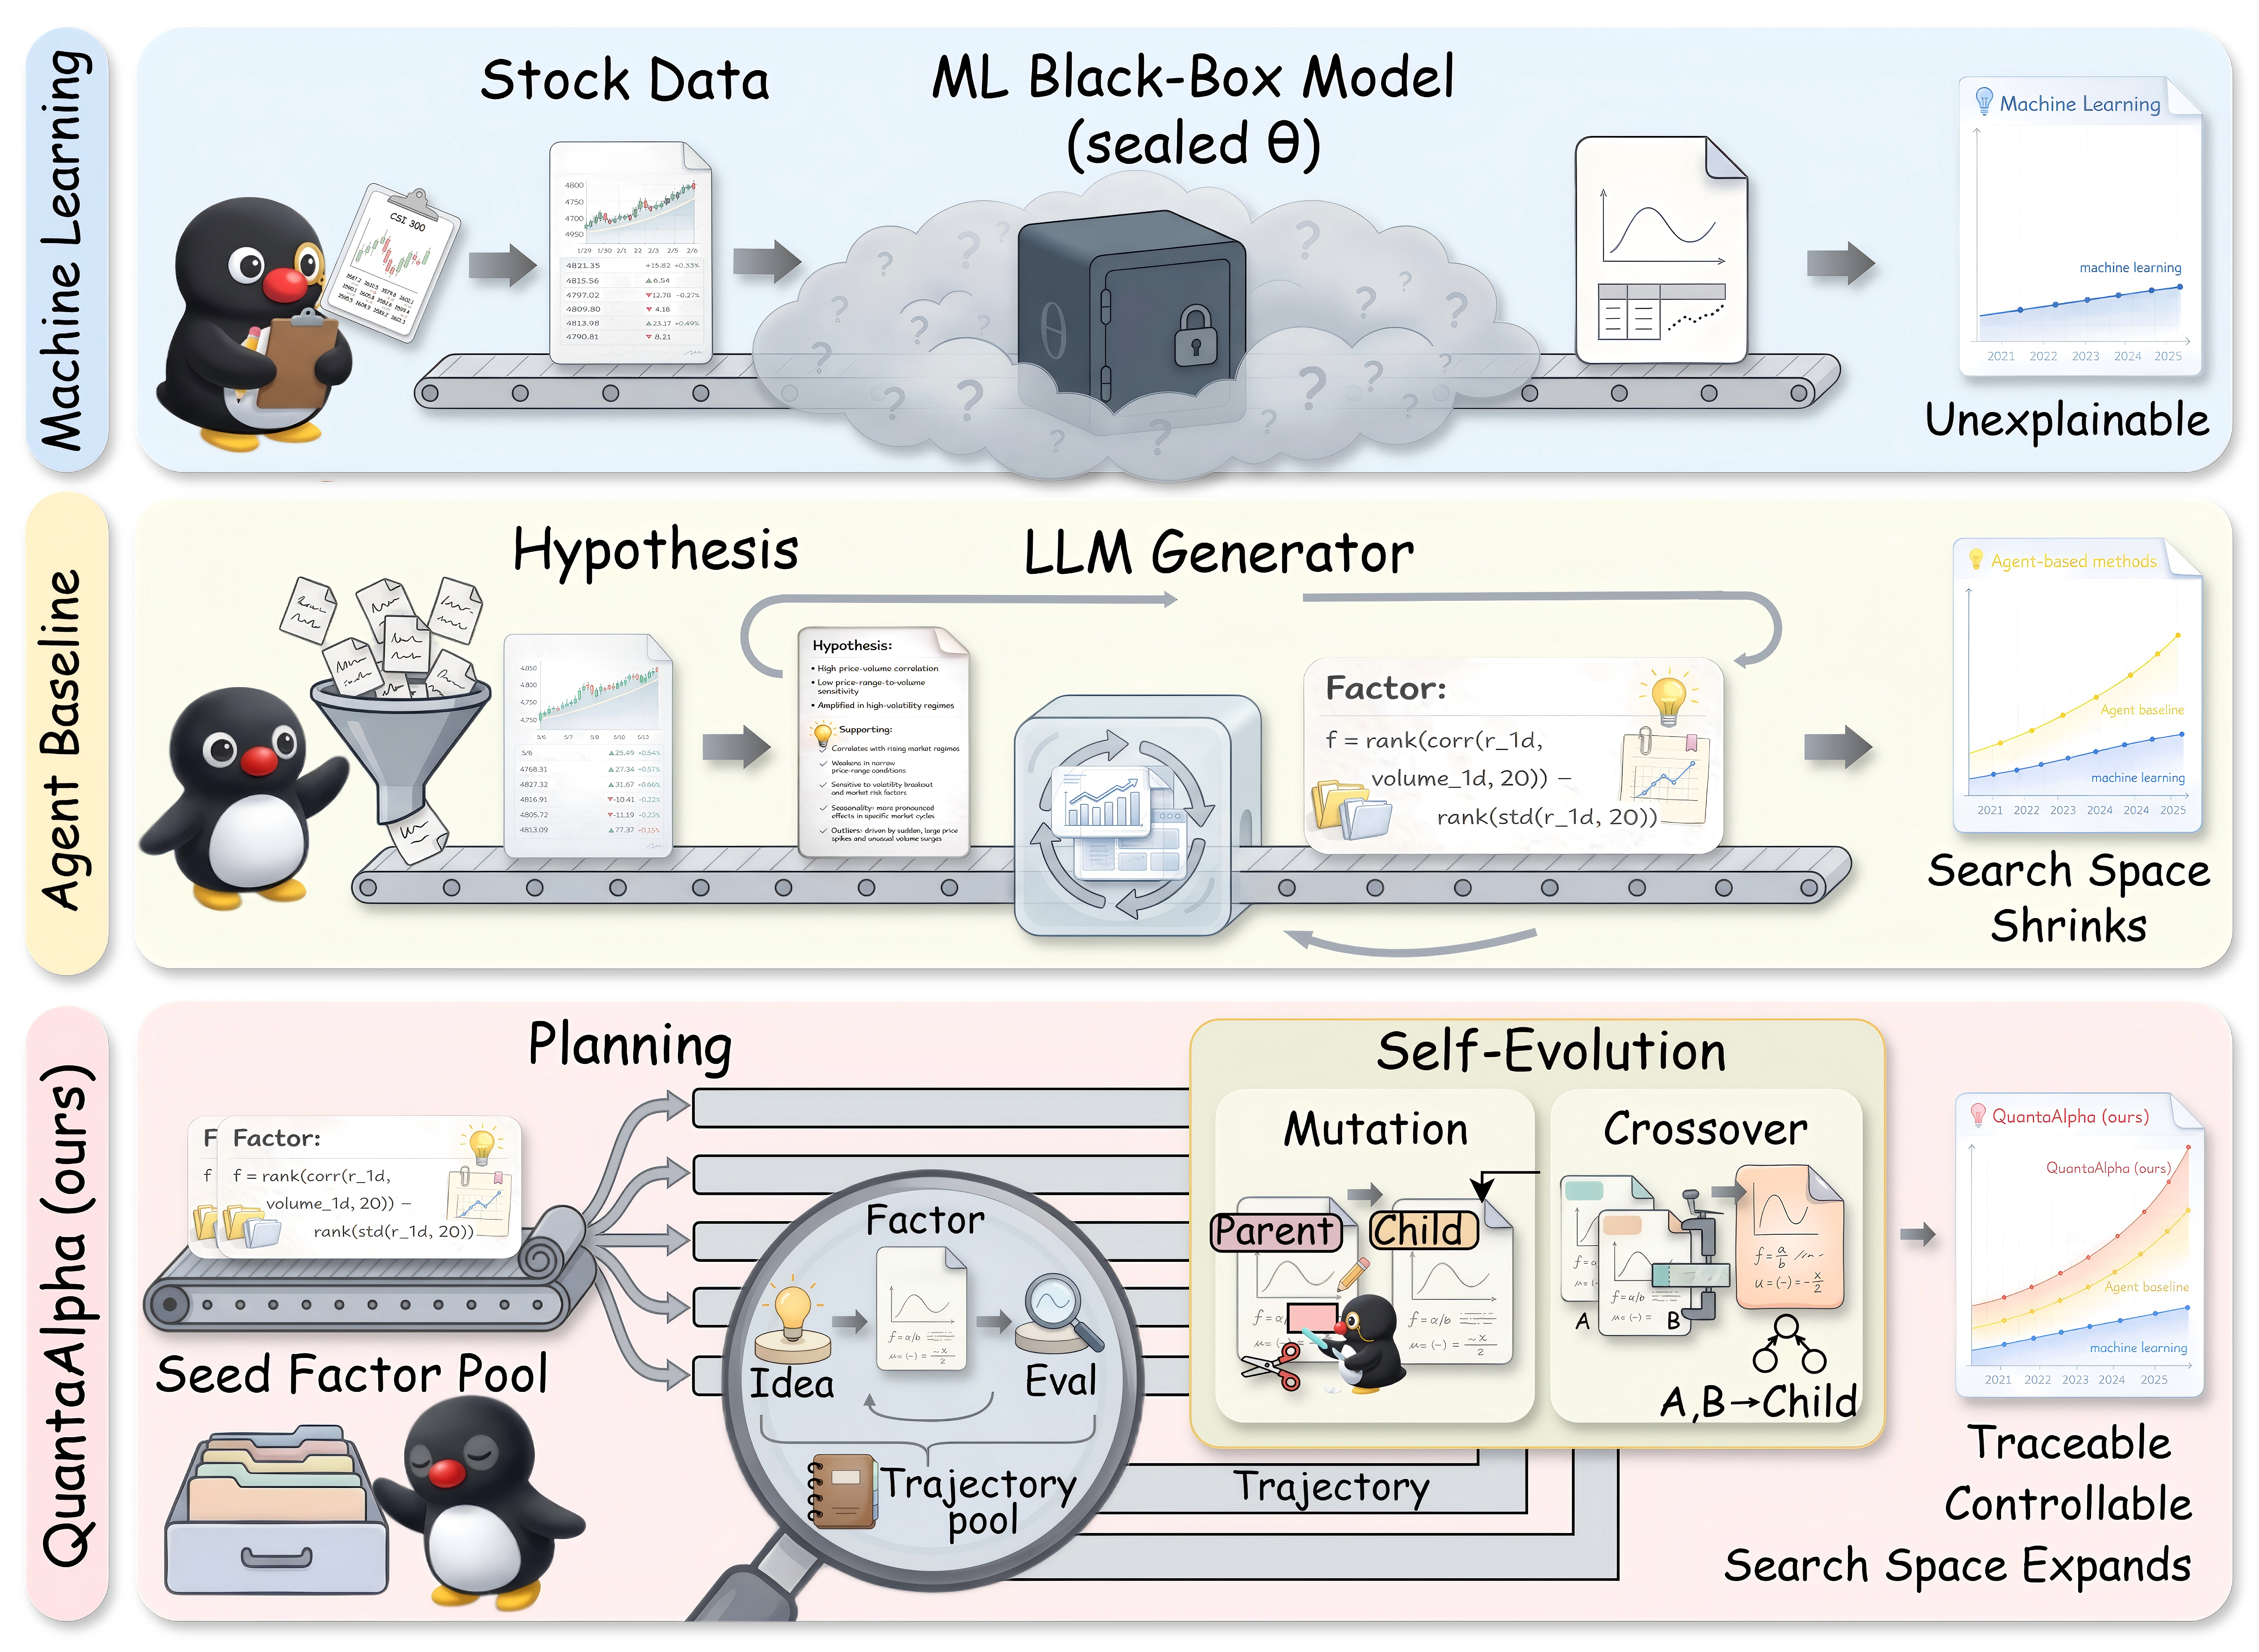
\includegraphics[width=0.8\linewidth]{images/Intro.jpg}
    \caption{Comparison with existing methods: QuantaAlpha improves alpha discovery through trajectory-level self-evolution.}
    \label{fig:placeholder}
\end{figure}
Representative agent frameworks for alpha mining simulate the workflow of human quantitative researchers by iteratively performing hypothesis generation, executable factor construction, and backtesting-based refinement, as illustrated in Figure~\ref{fig:placeholder}. Under this paradigm, AlphaAgent \cite{Tang2025AlphaAgent} imposes explicit regularization during factor generation to curb factor crowding and mitigate alpha decay, while RD-Agent \cite{li2025rdagent} targets full-stack automation with coordinated research and development agents, enabling joint factor–model co-optimization for robust strategy discovery. These frameworks reduce the trial-and-error costs of factor research while preserving interpretability relative to parameter-trained methods, making large-scale exploration practical.

However, under real-market non-stationarity and low signal-to-noise ratios, existing systems still face three limitations. \textit{(i) Fragile controllability:} Iterative refinement is driven by noisy backtest feedback, which can induce semantic drift and steer updates toward spurious correlations, gradually deviating from the intended economic mechanism. \textit{(ii) Limited trustworthiness:} Many methods rely on stochastic re-generation conditioned on transient contexts, without explicitly inheriting validated rationales across iterations. As a result, they lack a traceable lineage and the produced factors are harder to audit and trust. \textit{(iii) Constrained exploration:} Search often over-exploits local neighborhoods around initial seeds, leading to redundancy and factor crowding, while providing limited systematic coverage of the broader hypothesis space and weakening long-horizon discovery. 

To address these challenges, we propose \method, an evolutionary alpha mining framework that improves factor quality through trajectory-level self-evolution. Inspired by \cite{lin2025se}, we view each end-to-end mining run as a mining trajectory and explicitly evolve trajectories rather than relying on unconstrained re-generation from noisy feedback. First, to mitigate local optimization, we introduce a Diversified Planning Initialization that generates multiple complementary research directions, yielding broad initial coverage in the hypothesis space. Second, to support controllable refinement and reliable reuse of validated experience, \method performs self-evolution via trajectory-level mutation and crossover. Mutation performs targeted revision by localizing the failure-causing step via self-reflection and rewriting only the corresponding segment, while keeping the rest of the trajectory intact. Crossover recombines complementary segments from high-reward parents to reuse validated hypothesis structures, construction patterns, and repair behaviors. We further apply generation constraints to enforce semantic consistency and constrain complexity and redundancy, preventing drift and crowding. Together, these mechanisms expand exploration while stabilizing refinement under real-market noise and non-stationarity. Extensive experiments on CSI 300 and cross-market transfer to CSI 500 and S\&P 500 demonstrate consistent improvements in predictive power and strategy performance over strong baselines and prior agentic systems.
\section{Related Work}

\paragraph{Agents in Finance} 
Recent advances in financial LLMs \citep{liu2023fingpt, liu2025fin} and evaluation benchmarks \citep{guo2025fineval, tang2025finmmr} have substantially expanded the scope of automated financial reasoning.
Building on these foundations, a growing line of work explores how agentic systems \citep{li2025investorbench, yang2026finvault} can move beyond financial understanding toward {decision-oriented research workflows}, including factor discovery and trading analysis.
In this context, the pursuit of alpha factors has evolved from manual engineering and heuristic search toward LLM-driven closed-loop discovery \cite{li2024can,shi2025navigating, chen2025alphasage, wang2025alpha}.
Beyond search optimization, recent efforts emphasize workflow systematization. RD-Agent \cite{li2025rdagent} proposes a multi-agent framework that decouples the pipeline into research and development stages, enabling data-centric joint optimization of factors and models. To address market non-stationarity, AlphaForge \cite{shi2024alphaforge} focuses on the dynamic combination of mined factors, 
while Alphafin \cite{li2024alphafin} and AlphaEval \cite{ding2025alphaeval} establish standardized, task-oriented protocols for reproducible evaluation. Despite these advances, trading constraints (e.g., turnover, complexity) remain largely post-hoc filters rather than intrinsic objectives, leading to suboptimal generalization and interpretability in live trading.
\paragraph{Self-Evolving Agents} Self-evolving agents \cite{fang2025comprehensive, zhai2025agentevolver, lin2025se, zhang2026evofsm} represent a paradigm shift from static instruction-following to autonomous learning through interacting with environment. 
AlphaEvolve \cite{novikov2025alphaevolve} demonstrates a coding-centric evolution where the agent employs evolutionary resampling to autonomously generate algorithms for scientific discovery. Building on this, CSE \cite{hu2026controlled} introduces controllable self-evolution, facilitating a critical transition from stochastic generation to feedback-driven evolution.
The financial domain adapts thi s self-evolutionary framework to handle non-stationary and high-dimensional data. Research has converged on multi-agent coordination and structured feedback to guide evolution \cite{li2025hedgeagents}. TradingAgents \cite{xiao2025trad} and FactorMAD \cite{duan2025factormad} utilize institutional-style debates to refine trading hypotheses, while QuantAgents \cite{li2025quantagents} and ATLAS \cite{papadakis2025atlas} incorporate simulated trading performance as a reward signal for dynamic prompt optimization. To ensure consistency over long horizons, FinMem \cite{yu2025finmem} and FinCon \cite{yu2024fincon} leverage hierarchical memory and conceptual reinforcement to retain and refine high-level trading experience.
Despite these advancements, the transition of self-evolving agents to finance is hindered by the low signal-to-noise ratio and non-stationary. To mitigate this, our \method employs stable optimization units with mutation and crossover operators, ensuring a robust, traceable evolution path through structured archiving of iteration logic.
  
\section{Problem Setup}
\paragraph{Alpha Mining}
The alpha mining task aims to learn an alpha factor $f$ from a market feature tensor $\mathbf{X}\in\mathbb{R}^{N\times T\times D}$ for a stock universe $\mathcal{S}=\{s_1,\ldots,s_N\}$ and a time horizon $\mathcal{T}=\{t_1,\ldots,t_T\}$. 
At each time $t\in\mathcal{T}$, the factor produces a signal from the feature slice $\mathbf{X}_t\in\mathbb{R}^{N\times D}$ that is used to predict the cross-sectional return $\mathbf{y}_{t+1}\in\mathbb{R}^{N}$.
In notation, an alpha can be written as $f(\mathbf{X}_t)\rightarrow \mathbf{y}_{t+1}$, where $\mathbf{y}_{t+1}$ denotes the realized returns at time $t+1$. Accordingly, we formulate alpha mining as the following optimization problem:
\begin{equation}
f^{*}=\arg\max_{f\in\mathcal{F}}\ \mathcal{L}\big(f(\mathbf{X}),\mathbf{y}\big)-\lambda\mathcal{R}(f),
\label{eq:alpha_mining}
\end{equation}
where $\mathcal{F}$ denotes the space of all possible factor expressions, $\mathbf{y}$ is the ground-truth return target (e.g., next-day returns), $\mathcal{L}(\cdot)$ measures predictive effectiveness, $\mathcal{R}(\cdot)$ is a regularization term that encourages simplicity and novelty of the expression, and $\lambda$ balances utility and regularization.
\paragraph{Alpha Mining Trajectory}
Distinct from purely data-driven pipelines, we introduce market hypotheses $h\in\mathcal{H}$ to guide LLM-based factor construction. 
Each alpha mining run follows an end-to-end workflow from hypothesis generation to factor generation and backtesting evaluation (see Section~\ref{sec:4.1}). 
We represent each run by a mining trajectory, defined as an ordered sequence $\tau=(s_0,a_0,s_1,a_1,\ldots,s_n)$, where $s_0$ denotes the initial mining context (e.g., market context and optional user-provided seeds), $a_i$ is the action taken at step $i$ by the multi-agent system, and $s_n$ is the terminal state containing the evaluated result of this run. The quality of a trajectory is measured by its terminal reward:
\begin{equation}
R(\tau)=\mathcal{L}\big(f_{\tau}(\mathbf{X}),\mathbf{y}\big)-\lambda\mathcal{R}(f_{\tau}),
\label{eq:traj_reward}
\end{equation}
where $f_{\tau}$ denotes the factor produced by trajectory $\tau$.
\paragraph{Objective} Our objective is to find a trajectory generation mechanism $\pi$ for the multi-agent system that maximizes the expected terminal reward of the generated mining trajectory: 
\begin{equation}
\pi^{*}=\arg\max_{\pi}\ \mathbb{E}_{\tau\sim \pi}\bigl[R(\tau)\bigr],
\label{eq:objective_policy}
\end{equation}
where $\tau\sim\pi$ denotes the trajectory induced by repeatedly applying $\pi$ from the initial state $s_0$.

\section{Method}

As illustrated in Figure~\ref{fig:overview}, our approach treats alpha mining as an agentic research workflow rather than a one-shot factor construction procedure. 
Given market context and user-provided seeds, a multi-agent system produces a complete mining trajectory that records hypothesis generation, controllable factor construction, code implementation, and backtesting-based evaluation. 
We first describe the end-to-end mining workflow that instantiates and evaluates a single trajectory (Section~\ref{sec:4.1}). 
Building on these evaluated trajectories, we then introduce an evolutionary optimization scheme that iteratively improves mining quality via a self-evolution process (Section~\ref{sec:4.2}).
\begin{figure}[htbp]
    \centering
    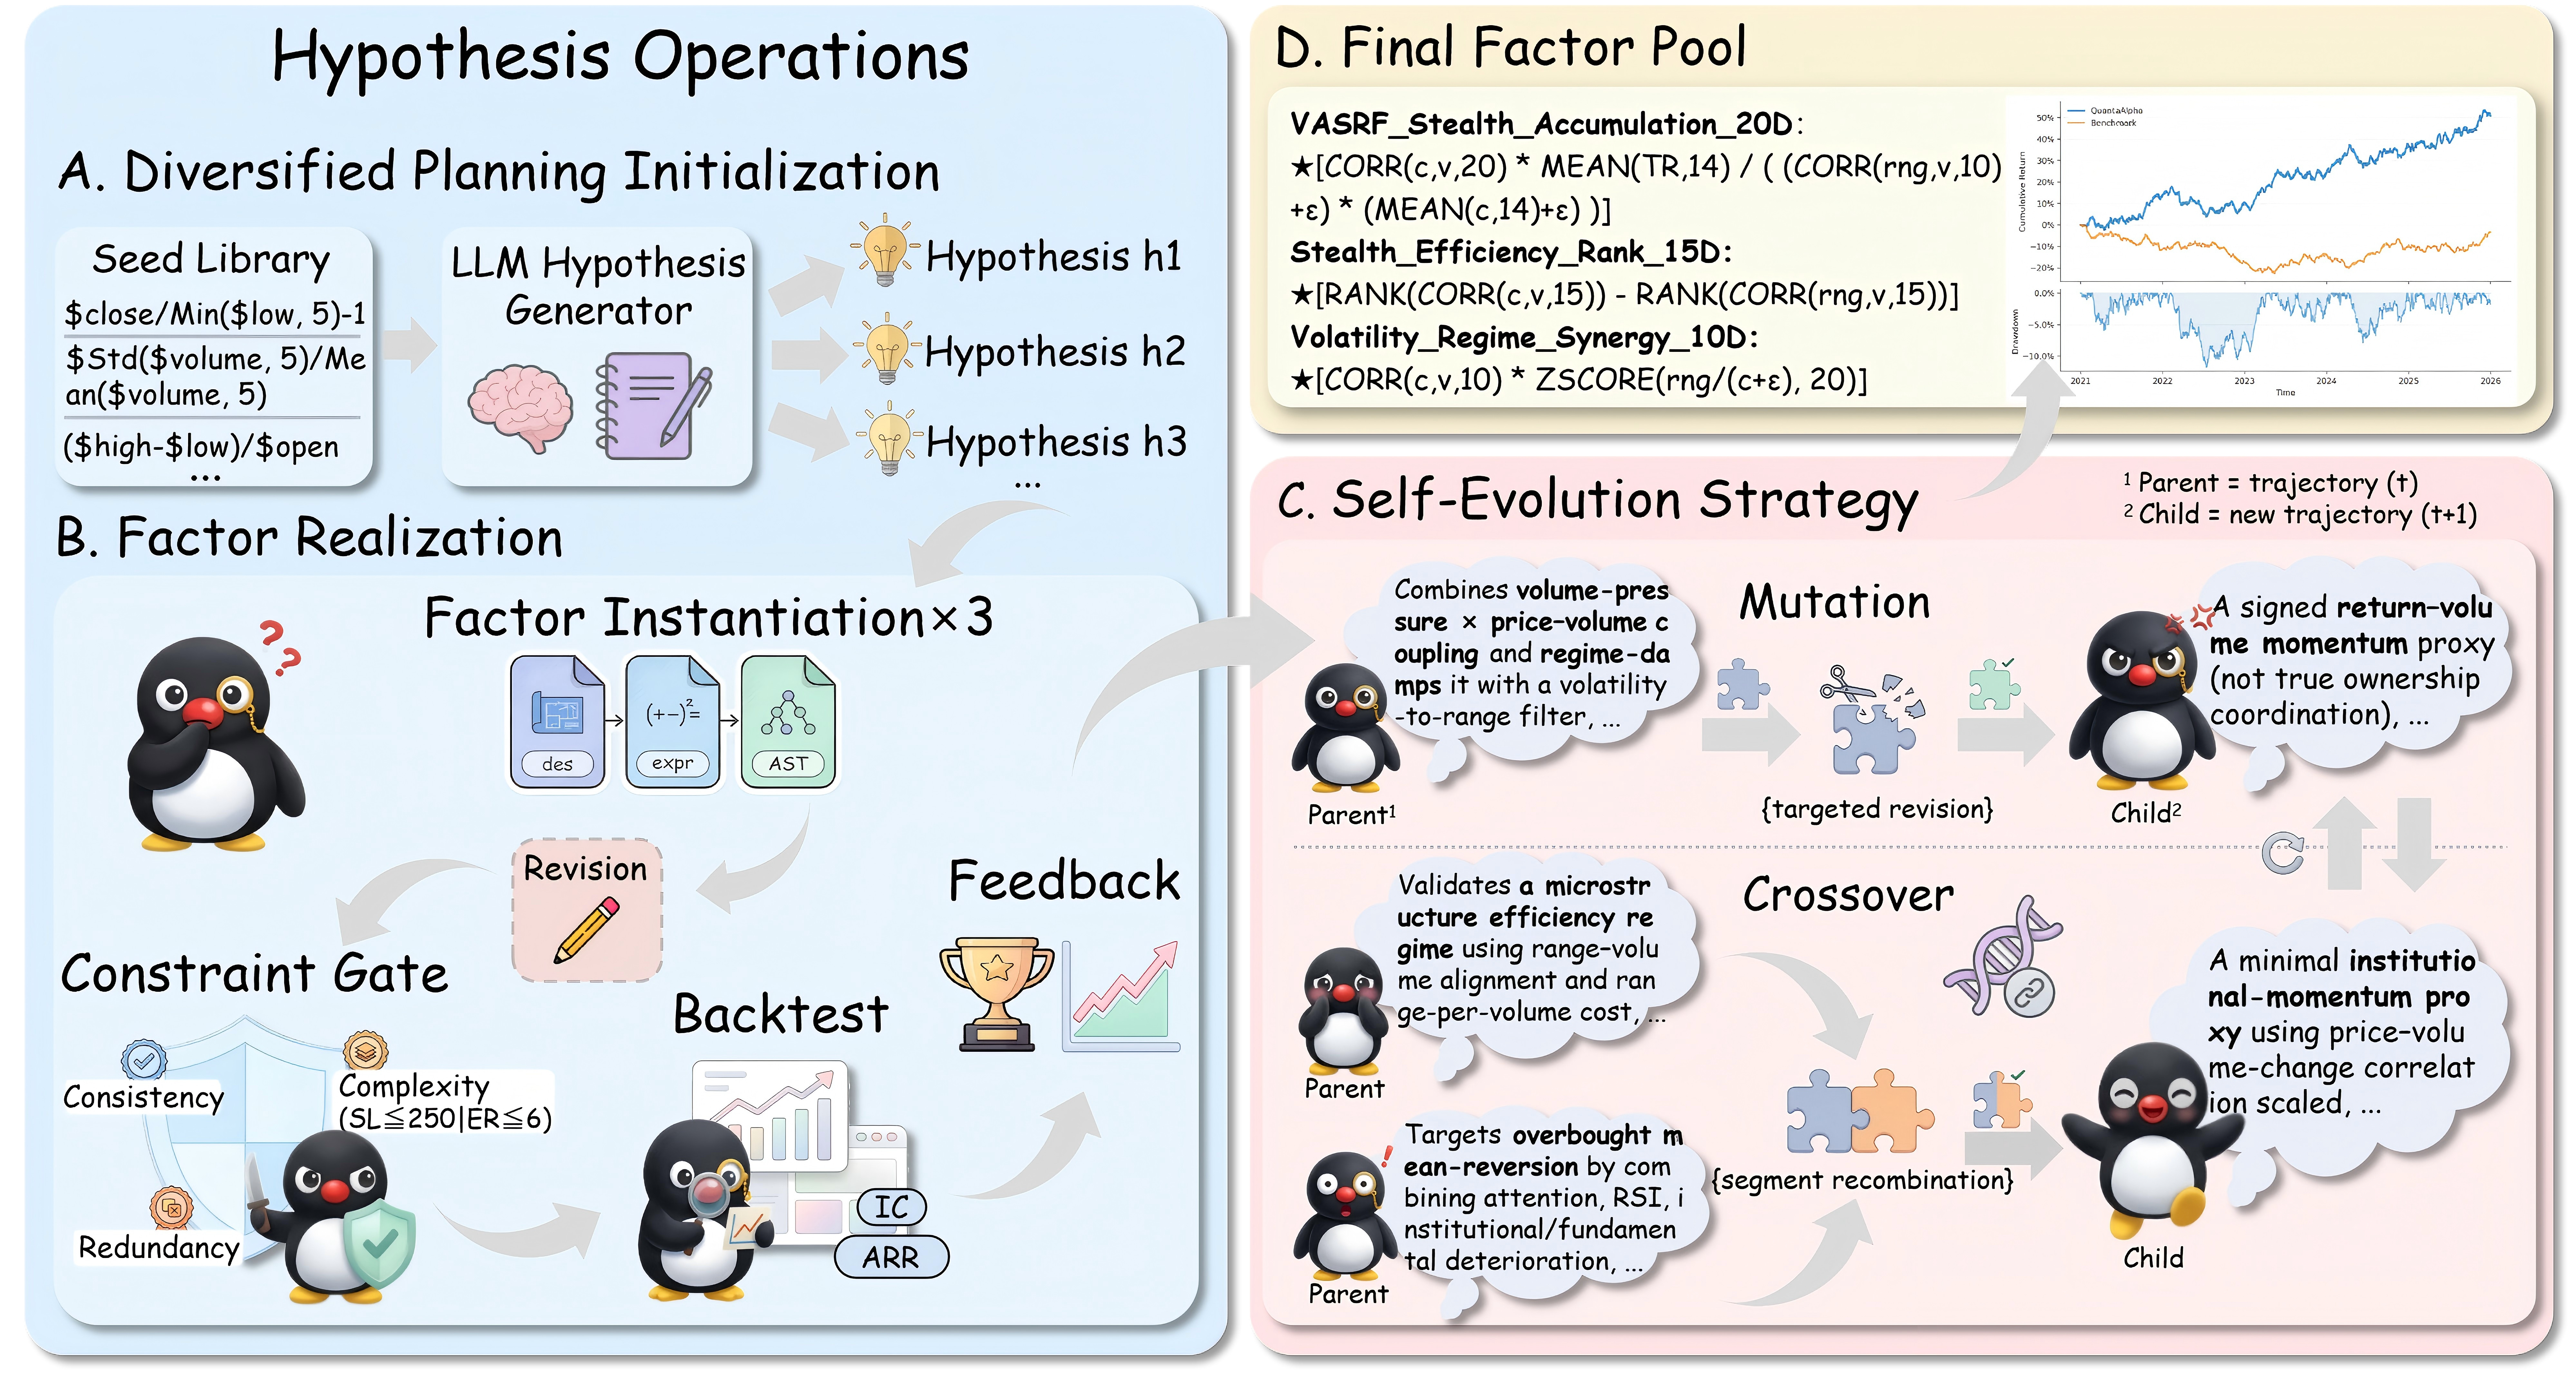
\includegraphics[width=1\textwidth]{images/overview.jpg}
    \caption{\textbf{Overview of the QuantaAlpha framework}. Our approach consists of four core components: (A) Diversified Planning Initialization to generate candidate hypotheses, (B) Factor Realization that iteratively instantiates hypotheses into executable factors with constraint gating, (C) Self-Evolution that applies mutation and crossover over evaluated trajectories, and (D) A Final Factor Pool that consolidates validated effective factors.}
    \label{fig:overview}
\end{figure}
\subsection{Alpha Mining Process} 
\label{sec:4.1}
A standalone alpha mining process involves a sequential progression starting from hypothesis generation, followed by factor creation and concluding with backtesting-based evaluation. We translate this process into the collaborative efforts of multiple agents, each responsible for a specific task at different stages of the workflow. 

\subsubsection{Hypothesis Generation}
We use the idea agent $\mathcal{A}{i}$ to generate market hypotheses via structured knowledge integration. Conditioned on (i) observations from current market conditions or previous mining trajectories, (ii) domain priors from financial theories and empirical evidence, and (iii) parametric specifications (e.g., ``10-day high/low''), $\mathcal{A}{i}$ produces actionable hypotheses that describe candidate market mechanisms and serve as the input to subsequent factor generation.

\subsubsection{Controllable Factor Construction}
To effectively instantiate hypothesis-driven factors, we need a robust mechanism to align implementations with domain hypotheses. However, directly generating factor code is brittle, often suffering from syntax errors, dependency mismatches, and semantic drift, causing a mismatch between the code and the hypothesis.To address these limitations, We introduce an intermediate symbolic representation based on a standardized operator library $\mathcal{O}$ and an Abstract Syntax Tree (AST). This abstraction bridges high-level market intent and low-level implementation, enabling controllable construction, structural validation, and reliable compilation.
\paragraph{Factor Generation} Given a hypothesis $h \in \mathcal{H}$ and raw features $\mathcal{X}$, the factor agent $\mathcal{A}_{f}$ generates a symbolic expression $f \in \mathcal{F}$ over the operator library and parses it into an AST as the intermediate representation. Concretely, it first maps $h$ to a structured semantic description $d$ that formalizes the intended mechanism into discrete operators, while concurrently instantiating operational parameters—such as look-back windows and thresholds—from either prescribed parameters in $h$ or heuristic defaults anchored in domain expertise.
Conditioned on $d$, the agent then assembles an operator composition into a symbolic expression $f$ and parses it into an AST, denoted as $T(f)$. In $T(f)$, leaf nodes bind to raw feature fields (e.g., \texttt{\$high}, \texttt{\$volume}) and internal nodes correspond to operator instances from $\mathcal{O}$ (e.g., \texttt{TS\_MIN}($\cdot$), \texttt{SMA}($\cdot$), \texttt{RANK}$(\cdot)$), thereby rendering the computational dependencies and data flow fully transparent.
Finally, the agent translates the validated symbolic form into executable code $c$ via compilation; when compilation fails due to implementation issues, an LLM-based repair step is triggered to regenerate a consistent implementation while preserving the semantics of $f$. This design ensures that code generation remains anchored to an explicit symbolic specification rather than unconstrained free-form generation.
\paragraph{Consistency Verification} We enforce semantic consistency across representations to prevent drift during generation. Specifically, we apply an LLM-based verifier to assess (i) alignment among the hypothesis $h$, semantic description $d$, and symbolic expression $f$, and (ii) faithfulness between the symbolic definition $f$ and the generated code $c$. The verifier returns a consistency decision under fixed criteria. If it fails, we rewrite the inconsistent component(s) by regenerating $d$ and $f$ or repairing $c$ until the check passes or a maximum retry budget is reached.
\paragraph{Complexity and Redundancy Control} We further regularize factor generation with explicit structural constraints to promote parsimony and novelty. For complexity, we compute
\begin{equation}
\mathcal{C}(f)
= \alpha_1 \cdot SL(f)
+ \alpha_2 \cdot PC(f)
+ \alpha_3 \cdot \log\!\bigl(1 + |F_f|\bigr),
\label{eq:factor_complexity}
\end{equation}
where $SL(f)$ measures symbolic length, $PC(f)$ counts free parameters (e.g., window sizes), and $F_f$ is the set of raw features used by $f$. For redundancy, we quantify structural similarity via AST matching. Given two factors $f_i$ and $f_j$ with ASTs $T(f_i)$ and $T(f_j)$, we define $s(f_i,f_j)$ as the size of their largest common isomorphic subtree:
\begin{equation}
s(f_i,f_j)
=\max_{\substack{S_i \subseteq T(f_i), S_j \subseteq T(f_j), S_i \cong S_j}} |V(S_i)|.
\end{equation}
Here, $S_i$ and $S_j$ range over subtrees of $T(f_i)$ and $T(f_j)$, respectively, $S_i \cong S_j$ denotes subtree isomorphism, and $|V(S_i)|$ is the number of nodes in $S_i$. For a candidate factor $f$, we compute its maximum similarity against an existing alpha zoo $\mathcal{Z}$ as 
\begin{equation}
S(f)=\max_{\phi\in\mathcal{Z}} s(f,\phi).
\label{eq:max_similarity}
\end{equation}
We reject and rewrite any factor that violates the prescribed complexity or redundancy limits, promoting parsimonious generation while avoiding near-duplicate structures.
\subsubsection{Factor Evaluation} 
The evaluation agent $\mathcal{A}_{e}$ assesses factors via a standardized backtesting system. The protocol covers three complementary aspects: predictive capability metrics for forecasting effectiveness, return performance metrics for profit-generating potential under a fixed execution setting, and risk control metrics for stability and robustness across market conditions. Beyond factor scoring, the agent maintains an evaluation history that records outcomes and summarizes systematic patterns among successful and failed factors.

\subsection{Evolutionary Alpha Mining}
\label{sec:4.2}
We improve alpha discovery via iterative optimization over mining trajectories. Starting from user-provided seed factors, we generate a diversified set of initial hypotheses. We then run the end-to-end mining workflow in Section~\ref{sec:4.1} to turn each hypothesis into an evaluated mining trajectory, forming an initial trajectory pool $\mathcal{T}_0=\{\tau_1^0,\tau_2^0,\ldots,\tau_{N_{init}}^0\}$. We then apply an iterative evolution process to obtain progressively improved factors.
\subsubsection{Diversified Planning Initialization}
\label{sec:4.2.1}
Let $\mathcal{Z}_0$ denote the user-provided seed factors (or seed ideas). 
We employ an initialization agent $\mathcal{A}_0$ to propose a diversified set of initial hypotheses $\mathcal{H}^{0}=\{h^{0}_1,\ldots,h^{0}_{N_{init}}\}$. The agent is instructed to maximize complementarity among hypotheses at both semantic and structural levels, e.g., varying signal sources (price vs.\ volume), time scales (short-term vs.\ long-term), and mechanism types (momentum vs.\ mean-reversion or regime-conditioned triggers). For each $h^{0}_i \in \mathcal{H}^{0}$, we run the mining workflow in Section~\ref{sec:4.1} and obtain a mining trajectory $\tau^{0}_i$.
This diversified initialization expands the effective search frontier by providing broad starting coverage in the hypothesis space. As a result, the subsequent evolutionary process can explore multiple promising regions in parallel, significantly reducing the risk of premature convergence to a suboptimal local optimum.
\subsubsection{Self-Evolution}
\label{sec:4.2.2}
The goal of self-evolutionary updates is to guide the alpha mining system to search for better trajectories based on existing ones. Specifically, we apply trajectory-level operators to existing mining trajectories to generate improved trajectories as demonstrations. These demonstrations provide imitation learning priors that bias subsequent trajectory generation toward effective decisions. In practice, we instantiate the update with two evolutionary primitives, Mutation and Crossover, which revise a single trajectory or recombine complementary sub-trajectories, respectively. Each iteration $i$ yields a new trajectory generation $\mathcal{T}_i$, and factor quality improves progressively across iterations (see Figure~\ref{fig:case_study} in Appendix for a case study).
\paragraph{Mutation}
Given a mining trajectory $\tau \in \mathcal{T}_{i-1}$, the primitive first performs self-reflection to diagnose sub-optimal decision node that most significantly accounts for the low terminal reward,
denoted by an index $k\in\{0,\ldots,n-1\}$. 
We then rewrite only the localized action (or a short local segment) while keeping the remaining steps unchanged:
\begin{equation}
\tau_{child}=\big(s_0,a_0,\ldots,s_k,\mathrm{Refine}(a_k),s_{k+1}',a_{k+1}',\ldots,s_n'\big), 
\label{eq:controlled_mutation}
\end{equation}
where the prefix up to $s_k$ is frozen, and the remaining steps are regenerated by the agent conditioned on this fixed prefix to preserve trajectory coherence. Depending on the localized fault, the rewrite may update the hypothesis, the symbolic expression under the operator library, or the compiled code, and can introduce mechanism-level changes such as altering the time scale, or adding regime conditions.
\paragraph{Crossover}
Crossover aims to exploit and inherit validated components by recombining complementary sub-trajectories from high-quality parents. At iteration $i-1$, we select a parent subset $\mathcal{P}_{i-1}\subseteq \mathcal{T}_{i-1}$ based on trajectory reward (Eq.~\ref{eq:traj_reward}). Given $k$ parent trajectories $\tau^{(1)},\ldots,\tau^{(k)}\in\mathcal{P}_{i-1}$, Crossover synthesizes a new child trajectory by composing high-performing segments from different parents:
\begin{equation}
\tau_{\mathrm{child}} = \mathrm{Crossover}\big(\tau^{(1)},\ldots,\tau^{(k)}\big).
\label{eq:crossover}
\end{equation}
Operationally, the primitive identifies specific trajectory segments that consistently contribute to high cumulative rewards—such as hypothesis templates, factor construction patterns, or strategic repair actions—and merges them into a single, highly coherent sequence.
This recombination mimics the human practice of combining complementary strengths from different solutions, while providing a more credible lineage by explicitly inheriting decisions that have been validated in previously successful trajectories.


\section{Experiments}
\begin{table}[h]
\centering
\caption{
Performance comparison of different methods on \textit{\textbf{CSI 300}}.
We report both \textit{factor predictive power} and \textit{strategy-level performance} metrics, where \textbf{higher$\uparrow$} values  indicate better performance for all metrics (with the exception of MDD).
For each method category, the best result in each column is highlighted in \textbf{bold},
while the second-best result is \underline{underlined}.
Across all methods, the overall best-performing method is highlighted with a light \colorbox[RGB]{236,244,252}{blue background}.
}
\label{tab:csi300_results}
\setlength\tabcolsep{3.2pt}
\fontsize{8.1pt}{10.5pt}\selectfont
\begin{tabular}{llcccccccc}
\toprule[1.5pt]

\multicolumn{2}{c}{\multirow{2}{*}{\textbf{Methods}}} 
& \multicolumn{4}{c}{Factor Predictive Power}
& \multicolumn{4}{c}{Strategy Performance} \\
\cmidrule(lr){3-6} \cmidrule(lr){7-10}

\multicolumn{2}{c}{} 
& \textbf{IC} & \textbf{ICIR} & \textbf{Rank IC} & \textbf{Rank ICIR} 
& \textbf{IR (SHR*)} & \textbf{CR} & \textbf{ARR (\%)} & \textbf{MDD (\%)$\downarrow$} \\
\midrule[0.8pt]
\rowcolor[RGB]{230, 230, 230}\multicolumn{10}{c}{\textit{\textbf{Classical Factor Mining}}} \\
% ---------------- Machine Learning ----------------
\multirow{6}{*}{\textbf{Machine Learning}}
& Linear 
& 0.0155 
& 0.1174 
& 0.0368 
& 0.2834 
& -0.3078 
& -0.1407 
& -2.67 
& 18.97 \\


& XGBoost 
& 0.0175 
& 0.1336 
& 0.0420 
& 0.3417 
& -0.5280 
& -0.1488 
& -4.24 
& 28.50 \\

& CatBoost 
& 0.0162 
& 0.1203 
& 0.0405 
& 0.3289 
& -0.2807 
& -0.1077 
& -2.30 
& 21.35 \\

& LightGBM 
& \underline{0.0247} 
& \underline{0.2055} 
& \underline{0.0423} 
& \underline{0.3726} 
& 0.0092 
& 0.0032 
& 0.07 
& 21.80 \\


& MLP 
& \textbf{0.0321} 
& \textbf{0.2780} 
& \textbf{0.0438} 
& \textbf{0.4088} 
& \underline{0.1716} 
& \underline{0.0804} 
& \underline{1.46} 
& \underline{18.15} \\


& DoubleEnsemble 
& 0.0213 
& 0.1670 
& 0.0408 
& 0.3372 
& \textbf{0.2490} 
& \textbf{0.1233} 
& \textbf{1.85} 
& \textbf{15.00} \\

\midrule
% ---------------- Deep Learning ----------------
\multirow{4}{*}{\textbf{Deep Learning}}
& GRU 
& 0.0321 
& 0.2603 
& 0.0442 
& 0.3601 
& 0.5302 
& 0.2405 
& 3.61 
& 15.01 \\

& Transformer 
& \underline{0.0331} 
& \underline{0.2702} 
& \underline{0.0451} 
& \underline{0.3801} 
& 0.4502 
& 0.3773
& 5.21
& \underline{13.81} \\


& LSTM 
& \underline{0.0331} 
& 0.2502 
& \underline{0.0451} 
& 0.3503 
& \underline{0.6802} 
& \underline{0.4058} 
& \underline{6.01} 
& 14.81 \\

& TRA 
& \textbf{0.0421} 
& \textbf{0.3402} 
& \textbf{0.0511} 
& \textbf{0.4203} 
& \textbf{1.0502} 
& \textbf{0.8002} 
& \textbf{6.81} 
& \textbf{8.51} \\

\midrule
% ---------------- Factor Libraries ----------------
\multirow{3}{*}{\textbf{Factor Libraries}}
& Alpha158(20) 
& 0.0051 
& 0.0329 
& 0.0184 
& 0.1177 
& \underline{0.5044} 
& 0.2087 
& \textbf{4.63} 
& 22.19 \\

& Alpha158 
& \textbf{0.0131} 
& \textbf{0.0817} 
& \textbf{0.0334} 
& \textbf{0.2119} 
& 0.4099 
& \underline{0.2620} 
& 2.66 
& \textbf{10.15} \\

& Alpha360 
& \underline{0.0105} 
& \underline{0.0636} 
& \underline{0.0306} 
& \underline{0.1889} 
& \textbf{0.6009} 
& \textbf{0.3550} 
& \underline{4.09} 
& \underline{11.52} \\

\midrule[0.8pt]
\rowcolor[RGB]{230, 230, 230}\multicolumn{10}{c}{\textit{\textbf{LLM-based Agentic Factor Mining}}} \\
% \rowcolor[RGB]{230, 230, 230}{\multicolumn{10}{c}{LLM-based Agent}}
% ---------------- LLM R&D Agent ----------------
\multirow{5}{*}{\textbf{RD-Agent}}
& Qwen3-235B 
& 0.0352 
& 0.2850 
& 0.0485 
& 0.3950 
& 0.6502 
& 0.3591 
& 7.20 
& 20.05 \\

& Deepseek-V3.2 
& 0.0401 
& 0.3250 
& 0.0522 
& 0.4250 
& 0.8202 
& 0.4332 
& 7.81 
& 18.03 \\

& Gemini-3-pro-preview 
& 0.0481 
& 0.3900 
& 0.0583 
& 0.4750 
& 1.0202 
& 0.5499 
& 8.81 
& 16.02 \\

& Claude-4.5-sonnet 
& \underline{0.0527} 
& \underline{0.4250} 
& \underline{0.0623} 
& \underline{0.5050} 
& \underline{1.2202} 
& \underline{0.6488} 
& \underline{9.81} 
& \underline{15.12} \\

& GPT-5.2 
& \textbf{0.0531} 
& \textbf{0.4300} 
& \textbf{0.0633} 
& \textbf{0.5150} 
& \textbf{1.2502} 
& \textbf{0.6687} 
& \textbf{9.91} 
& \textbf{14.82} \\
\midrule
% ---------------- AlphaAgent ----------------
\multirow{5}{*}{\textbf{AlphaAgent}}
& Qwen3-235B 
& 0.0952 
& 0.6632 
& \underline{0.1019} 
& \underline{0.6471} 
& \underline{2.1053} 
& \underline{1.5945} 
& 15.10 
& \underline{9.47} \\

& Deepseek-V3.2 
& 0.0955 
& \underline{0.6637} 
& 0.0919 
& 0.6450 
& 1.9230 
& 1.4746 
& 14.51 
& 9.84 \\

& Gemini-3-pro-preview 
& 0.0804 
& 0.5366 
& 0.0784 
& 0.5290 
& 1.7821 
& 1.4729 
& 14.11 
& 9.58 \\

& Claude-4.5-sonnet 
& \textbf{0.1092} 
& \textbf{0.7718} 
& \textbf{0.1062} 
& \textbf{0.7596} 
& \textbf{2.2739} 
& \textbf{2.0246} 
& \textbf{16.48} 
& \textbf{8.14} \\

& GPT-5.2 
& \underline{0.0966} 
& 0.6344 
& 0.0942 
& 0.6237 
& 1.9328 
& 1.2056 
& \underline{15.54} 
& 12.89 \\

\midrule
% ---------------- QuantaAlpha ----------------
\multirow{5}{*}{\colorbox[RGB]{245, 235, 235}{\textbf{QuantaAlpha}}}
& Qwen3-235B 
& 0.1252 
& \underline{0.8672} 
& 0.1226 
& \underline{0.8577}
& 2.6114 
& 2.2859 
& 20.55 
& 8.99 \\

& Deepseek-V3.2 
& \underline{0.1338} 
& 0.8533 
& \underline{0.1300} 
& 0.8304
& \underline{2.8797} 
& 2.6007 
& \underline{23.77} 
& 9.14 \\





& Gemini-3-pro-preview 
& 0.1124 
& 0.7391 
& 0.1086 
& 0.7205 
& 2.5189 
& 2.1503 
& 20.32 
& 9.45 \\

& Claude-4.5-sonnet 
& 0.1111 
& 0.6374 
& 0.1077 
& 0.6211 
& 2.6459 
& \underline{3.2615} 
& 22.70 
& \colorbox[RGB]{236,244,252}{\textbf{6.96}} \\

& GPT-5.2 
& \colorbox[RGB]{236,244,252}{\textbf{0.1501}}
& \colorbox[RGB]{236,244,252}{\textbf{0.9110}}
& \colorbox[RGB]{236,244,252}{\textbf{0.1465}} 
& \colorbox[RGB]{236,244,252}{\textbf{0.8909}}
& \colorbox[RGB]{236,244,252}{\textbf{3.3251}}
& \colorbox[RGB]{236,244,252}{\textbf{3.4774}}
& \colorbox[RGB]{236,244,252}{\textbf{27.75}}
& \underline{7.98} \\


\bottomrule[1.5pt]
\end{tabular}
\end{table}









%  \begin{table}[tb]
%   \centering
%   \small
%   \caption{Ablation Study Results of QuantaAlpha's Constrain Gate Mechanisms}
%   \label{tab:constrain_gate_ablation}
%   \resizebox{\linewidth}{!}{
%     \begin{tabular}{l|ccc|cccccc}
%       \hline
%       \multirow{2}{*}{Model Variant} & \multicolumn{3}{c|}{Constrain Gate Mechanisms} & \multicolumn{6}{c}{Key Metrics} \\
%       \cline{2-10}
%       & Complexity Check & Redundancy Check & Consistency Check & IC & ICIR & ARR (\%) & IR (SHR*) & MDD (\%) & CR \\
%       \hline
%       QuantaAlpha (Full) & √ & √ & √ & \textbf{0.1494} & \textbf{0.9263} & \textbf{28.99} & \textbf{3.4828} & \textbf{-9.42} & \textbf{3.0763} \\
%       w/o Complexity Check & × & √ & √ & 0.1303 & 0.8173 & 23.51 & 2.7780 & -9.75 & 2.4113 \\
%       w/o Redundancy Check & √ & × & √ & 0.1252 & 0.8672 & 20.55 & 2.6114 & -11.99 & 1.7139 \\
%       w/o Consistency Check & √ & √ & × & 0.1223 & 0.8033 & 17.51 & 2.0776 & -10.69 & 1.6380 \\
%       \hline
%     \end{tabular}
%   }
%   \begin{tablenotes}
%     \small
%     \item  "w/o " denotes mechanism ablation; 
%   \end{tablenotes}
% \end{table}

\subsection{Experimental Setup}

\paragraph{Datasets and Metrics} We conduct experiments on the CSI 300 dataset, which covers 300 large-cap A-share stocks in the Chinese market. We adopt a chronological split with training (Jan. 1, 2016 to Dec. 31, 2020), validation (Jan. 1, 2021 to Dec. 31, 2021), and testing (Jan. 1, 2022 to Dec. 26, 2025). We evaluate performance from two complementary perspectives. Factor predictive power is measured by Information Coefficient (IC), IC Information Ratio (ICIR), Rank IC, and Rank ICIR. Strategy performance is measured by Annualized Return (ARR), Information Ratio (IR), Maximum Drawdown (MDD), and Calmar Ratio (CR). Further details are provided in Appendix~\ref{appendix:A.2}.

\paragraph{Baselines} We compare QuantaAlpha against four baseline categories: traditional machine learning models, deep learning time-series models, classical factor libraries, and LLM-based factor research agents, including RD-Agent and AlphaAgent. More details are provided in Appendix~\ref{appendix:A.5}.

\subsection{Main Results}
Table~\ref{tab:csi300_results} reports the main results on the CSI 300 market over a four-year evaluation period. QuantaAlpha outperforms all baselines on both factor predictive power and strategy-level performance. Using GPT-5.2, QuantaAlpha achieves the best IC at 0.1501, delivers an ARR of 27.75\%, and maintains a low MDD of 7.98\%. From a real-world perspective, this performance indicates that the mined factors can support production trading under standard risk controls, rather than being artifacts of backtest noise. Similarly, we observe consistent gains across different base models, suggesting that the improvements are robust rather than model-specific.

Compared with RD-Agent, QuantaAlpha and AlphaAgent both incorporate generation-stage regularization, and this is reflected in stronger predictive power and strategy performance. Under GPT-5.2, QuantaAlpha improves IC by 0.0970 and ARR by 17.84\% relative to RD-Agent while reducing MDD by 6.84\%, suggesting that constraining hypothesis-to-factor construction with explicit intermediate representations and verification effectively reduces semantic drift and improves implementation reliability. Beyond these constraints, QuantaAlpha further improves upon AlphaAgent by 0.0535 IC and 12.21\% ARR while reducing MDD by 4.91\%, highlighting the added value of trajectory-centric self-evolution: mutation broadens exploration via mechanism-level variations, while crossover reuses validated trajectory segments and repair strategies, jointly increasing the yield and stability of high-quality factors under non-stationary market dynamics.

\begin{figure}[t]
  \centering
  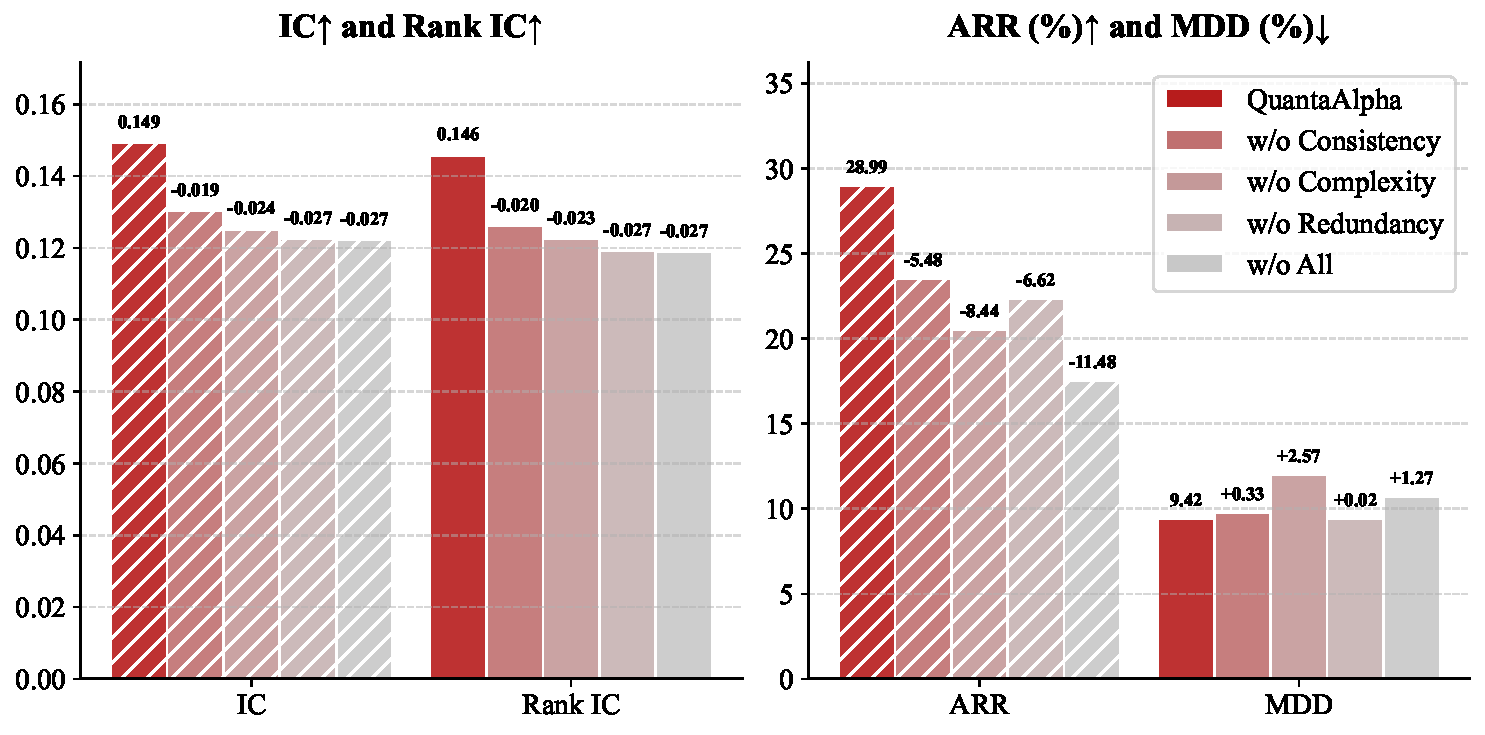
\includegraphics[width=0.8\columnwidth]{images/ablation.pdf}
  \caption{Ablation study of semantic consistency, complexity, and redundancy controls.}
  \label{fig:gate_ablation}
\end{figure}

\subsection{Ablation Study}
\paragraph{Ablation of Evolutionary Mining Components} We conduct an ablation study to quantify the contribution of three components in evolutionary alpha mining: diversified planning initialization, trajectory mutation, and trajectory crossover. The results are summarized in Table~\ref{tab:ablation_study_two_column}. Removing \emph{planning} yields only marginal changes in IC and Rank IC, but substantially degrades strategy-level outcomes, with ARR decreasing by 7.78\% and MDD increasing by 2.73\%. This indicates that diversified initialization primarily improves the search frontier by providing broader and less correlated starting hypotheses, which stabilizes subsequent evolution. In contrast, removing \emph{mutation} causes the largest drop in predictive power, decreasing IC by 0.0292 and Rank IC by 0.0284, and also leads to the largest reduction in ARR by 9.81\%. This highlights mutation as the primary driver of effective exploration and trajectory repair, enabling the system to escape suboptimal regions and correct failure modes discovered during mining. Meanwhile, removing \emph{crossover} leads to a smaller but consistent degradation. This supports the role of crossover in exploiting and inheriting complementary high-performing trajectory segments, improving efficiency and stability by recombining validated patterns from successful trajectories.
\begin{table}[h]
  \centering
  \normalsize % 核心跨档放大：从\scriptsize直接升级为\normalsize（文档默认正文字体，单栏表格大幅放大的最优选择）
  \caption{Ablation study of evolutionary mining components.}
  \label{tab:ablation_study_two_column}
  \setlength{\tabcolsep}{10pt} % 大幅舒展列间距（适配\normalsize字体，单栏下不超界且不冗余）
  \begin{tabular}{lcccc}
    \toprule
   \multirow{2}{*}{Method} & \multicolumn{4}{c}{Key Metrics} \\
    \cmidrule(lr){2-5}
     &  \multicolumn{1}{l}{\,\,\,\textbf{IC}} &  \multicolumn{1}{l}{\textbf{Rank IC}} &  \multicolumn{1}{l}{\textbf{ARR}} (\%) & \textbf{MDD} (\%) $\downarrow$\\
    \midrule

     \textbf{QuantaAlpha}
& \multicolumn{1}{l}{\textbf{0.1493}}
& \multicolumn{1}{l}{\textbf{0.1458}}
& \multicolumn{1}{l}{\textbf{28.99}}
& \multicolumn{1}{l}{\,\,\,\,\textbf{9.42}} \\

     \phantom{Q} -  \emph{w/o} \textbf{Planning}
      & 0.1488\textsuperscript{\textcolor[RGB]{230,180,180}{\tiny -0.0005}}
      & 0.1452\textsuperscript{\textcolor[RGB]{230,180,180}{\tiny -0.0006}}
      & 21.21\textsuperscript{\textcolor[RGB]{180,20,20}{\tiny -7.78}}
      & 12.15\textsuperscript{\textcolor[RGB]{200,50,50}{\tiny +2.73}} \\

     \phantom{Q} -  \emph{w/o} \textbf{Mutation}
      & 0.1201\textsuperscript{\textcolor[RGB]{180,60,60}{\tiny -0.0292}}
      & 0.1174\textsuperscript{\textcolor[RGB]{180,60,60}{\tiny -0.0284}}
      & 19.18\textsuperscript{\textcolor[RGB]{160,20,20}{\tiny -9.81}}
      & 9.85\textsuperscript{\textcolor[RGB]{220,160,160}{\tiny +0.43}} \\

      \phantom{Q} -  \emph{w/o} \textbf{Crossover}
      & 0.1423\textsuperscript{\textcolor[RGB]{220,150,150}{\tiny -0.0070}}
      & 0.1381\textsuperscript{\textcolor[RGB]{220,150,150}{\tiny -0.0077}}
      & 26.17\textsuperscript{\textcolor[RGB]{200,50,50}{\tiny -2.82}}
      & 10.63\textsuperscript{\textcolor[RGB]{220,100,100}{\tiny +1.21}} \\

    \bottomrule
  \end{tabular}
\end{table}


\paragraph{Ablation of Consistency, Complexity, and Redundancy Controls} We ablate three controls during factor generation that gate rewriting, including semantic consistency verification, complexity regularization, and redundancy filtering. As shown in Figure~\ref{fig:gate_ablation}, disabling any single control consistently degrades performance, confirming that each contributes non-trivially to robust factor generation. The \emph{consistency} control prevents semantic drift between the hypothesis, symbolic specification, and implementation. The \emph{complexity} control improves robustness by discouraging overly complex expressions that generalize poorly, and its removal leads to the most pronounced degradation at the strategy level, with the annualized excess return dropping by 8.44\% and the maximum drawdown increasing by 2.57\%. The \emph{redundancy} control preserves exploration by filtering near-duplicate structures and mitigating factor crowding. Disabling all three yields the largest degradation, indicating that these controls are complementary and jointly needed for reliable generation.

\subsection{More Analysis}

\paragraph{Factor Generalizability} To evaluate factor robustness under significant market distribution shifts, we conduct a zero-shot transfer experiment where the factors mined and selected on CSI 300 are directly deployed on CSI 500 and the S\&P 500 without any re-optimization or market-specific adaptation. As shown in Figure~\ref{fig:cumulative_returns}, QuantaAlpha demonstrates substantially stronger out-of-distribution generalization than all baselines. A clear divergence emerges around December 2023, when competing methods begin to stagnate under shifts in market microstructure and volatility regimes, whereas QuantaAlpha sustains a stable upward trajectory. By the end of the evaluation period, it reaches a cumulative excess return of roughly \textbf{160\%} on CSI 500 and over \textbf{137\%} on the S\&P 500. These results indicate that the discovered factors transfer beyond the source market and retain effectiveness under distribution shifts, rather than relying on market-specific historical patterns.

\paragraph{Alpha Decay} Figure~\ref{fig:annual_ic_rankic} reports annual IC and Rank IC on the CSI~300 universe from 2021 to 2025. A pronounced performance collapse is observed for the baselines in 2023, coinciding with a major regime shift in the A-share market. The pre-2023 period is dominated by large-cap ``core assets'', where institutional trading supports relatively stable trends and makes classical momentum or mean-reversion signals effective. In 2023, the market rotates toward small-cap and thematic stocks, together with higher intraday noise, more frequent overnight gaps, and weaker trend persistence. Baseline methods, whose factor libraries implicitly assume smooth trends and regular reversal patterns, fail to transfer to this out-of-distribution environment. QuantaAlpha, by comparison, maintains strong IC and Rank IC through the regime transition. It discovers more structural factors, such as \textit{Mean-Reverting Range Deviation} and \textit{Overnight Gap Structure}, that reflect persistent microstructure effects including volatility clustering and overnight information incorporation. These signals are less sensitive to capitalization style, enabling better temporal generalization. 
\begin{figure}[h]
\centering
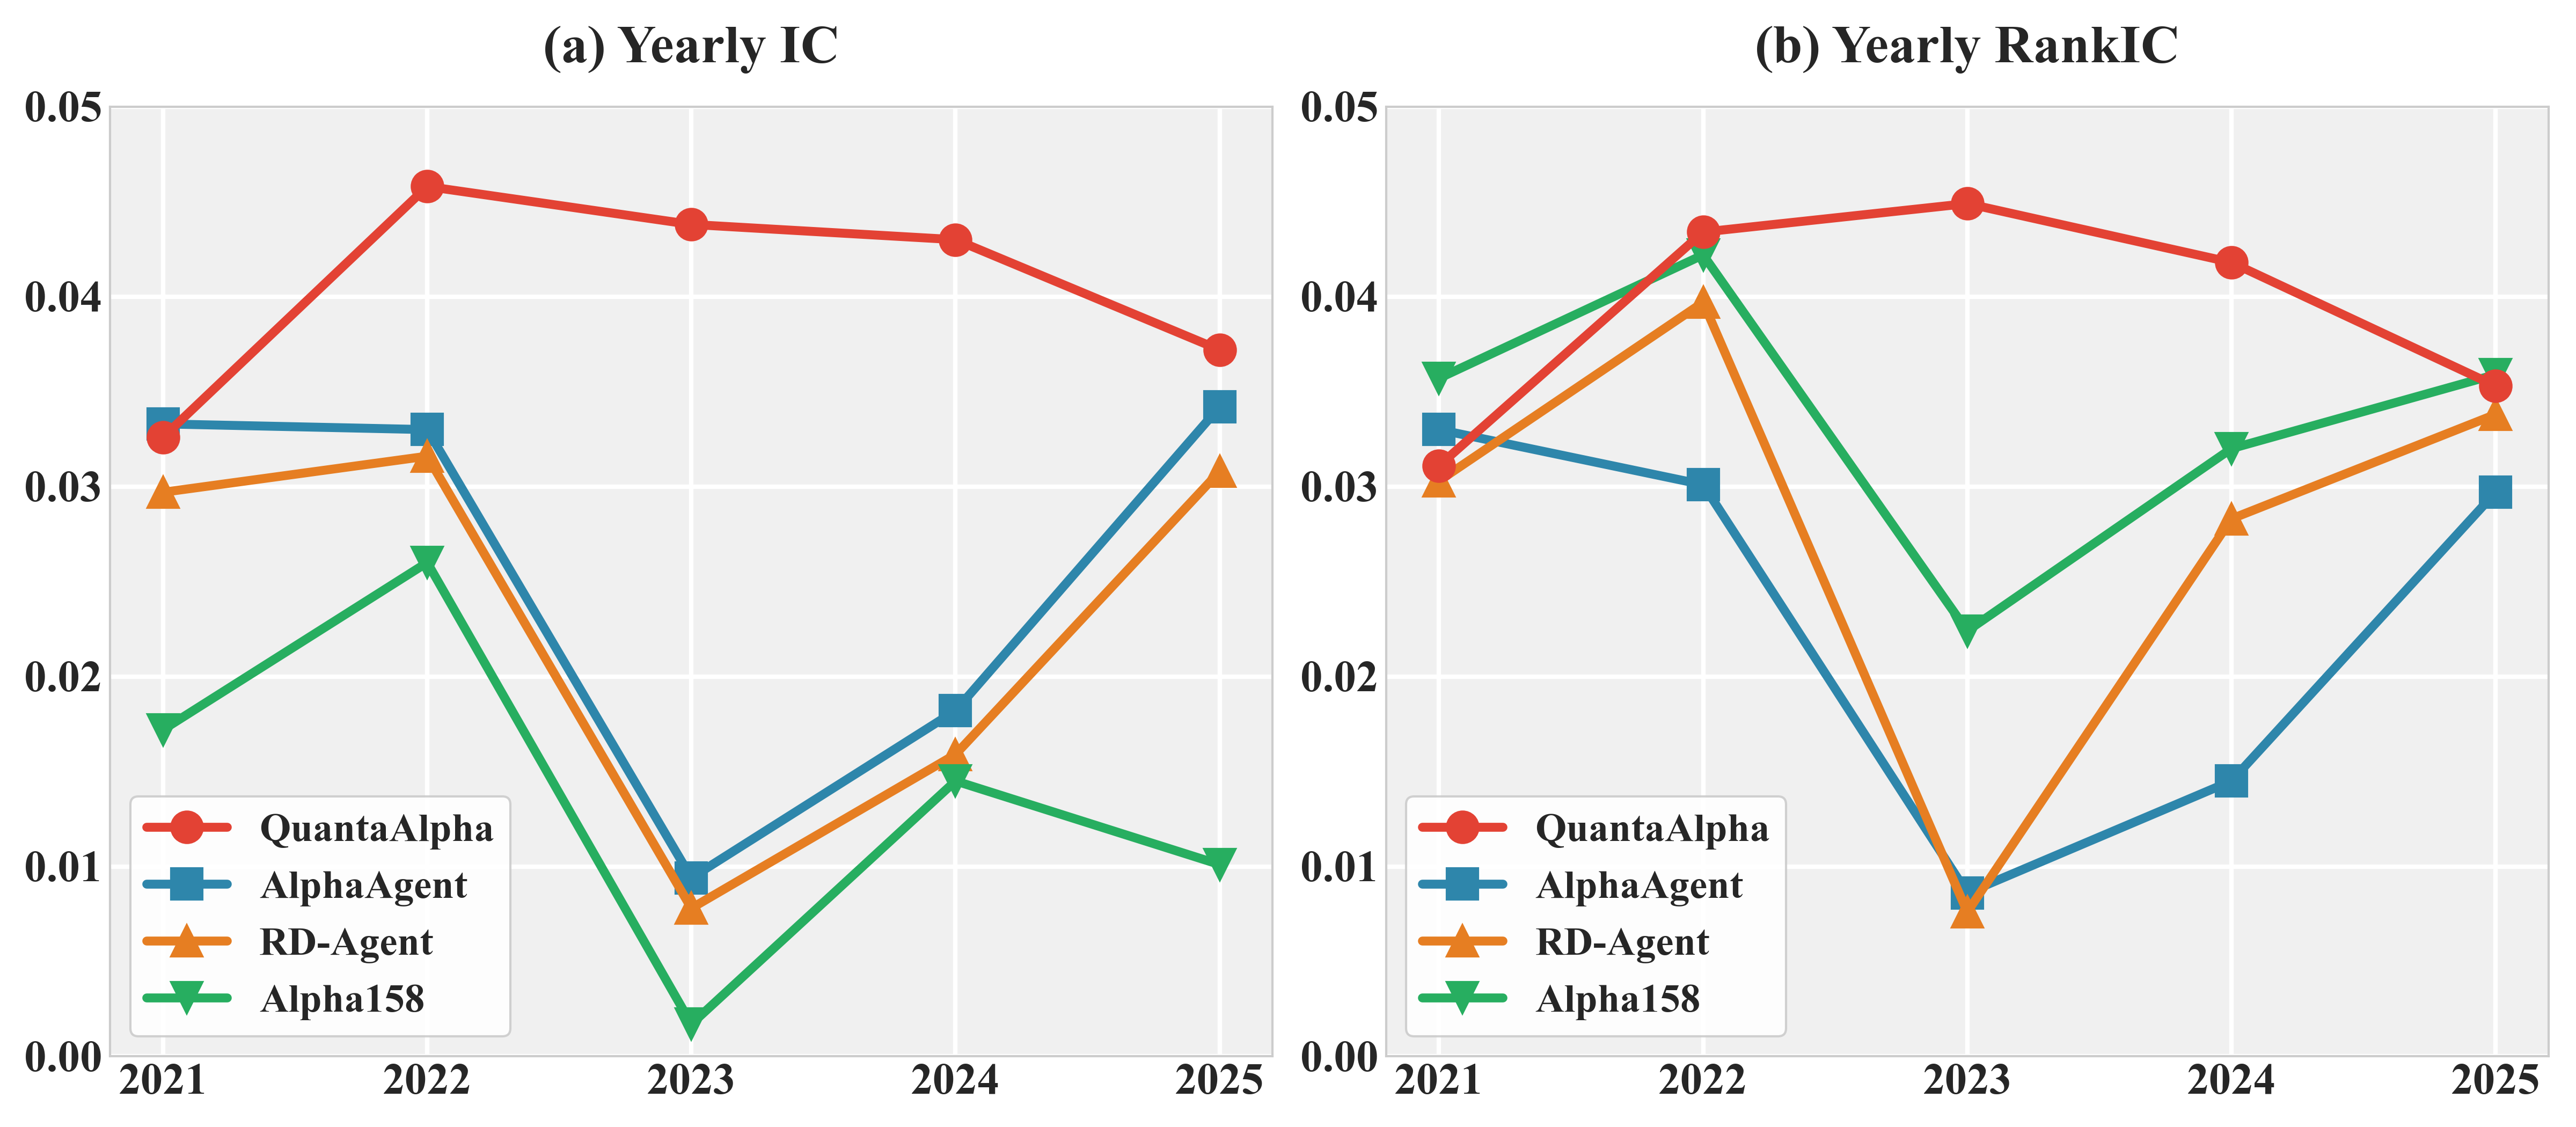
\includegraphics[width=0.8\columnwidth]{images/figure4.png} 
\caption{Annual IC and Rank IC comparison on the CSI 300.}
\label{fig:annual_ic_rankic}
\end{figure}

Table~\ref{tab:qa_aa_2023_representative} provides a factor-level diagnosis of the alpha decay observed in 2023, grounding the analysis jointly in \emph{market style changes}, \emph{factor semantics}, and \emph{empirical factor statistics}.  
Rather than enumerating factor formulas, we focus on which information channels remain predictive under the 2022--2023 regime transition and why.

\paragraph{Market Style Transition and Its Implications}

The CSI~300 market undergoes a pronounced style transition in 2023 relative to the training period (2016--2020).  
The earlier regime is dominated by large-cap core assets, with high institutional participation, smooth intraday dynamics, and persistent short-horizon trends. Under such conditions, classical momentum, mean-reversion, and exhaustion-based factors are effective.In 2023, leadership rotates toward small-cap and thematic stocks. This shift is accompanied by increased intraday noise, frequent overnight gaps driven by call auctions, and rapid cross-style liquidity re-allocation. These changes weaken trend persistence and amplify path-dependent noise, directly challenging factor constructions that rely on stable intraday structure or fast mean reversion.

\paragraph{Factor Semantics Aligned with Market Microstructure}

The empirical contrast between QuantaAlpha (QA) and AlphaAgent (AA) in 2023 reflects differences in the \emph{semantic composition} of their factor libraries.

\textbf{(i). Overnight and auction information.}
Gap-based factors aggregate information released during non-trading hours and price discovery in the opening auction.  
As shown in Table~\ref{tab:qa_aa_2023_representative}, multiple QA factors from this channel occupy the right tail of the 2023 Rank IC distribution, while maintaining near-complete coverage (Table~\ref{tab:qa_aa_2023_summary}). This indicates that overnight information becomes a dominant and stable signal when intraday predictability deteriorates.

\begin{table*}[!t] \centering \caption{Representative factors and their performance metrics on the CSI 300 index in 2023.} \label{tab:qa_aa_2023_representative} \scriptsize \setlength{\tabcolsep}{3pt} \renewcommand{\arraystretch}{1.06} \begin{tabular}{p{5.8cm}ccp{8.2cm}} \toprule \textbf{Factor (representative)} & \textbf{Rank IC} & \textbf{IC} & \textbf{Interpretation (short)} \\ \midrule \multicolumn{4}{c}{\textit{QA --- strong performers (overnight/auction, trend-quality, and liquidity re-rating)}} \\ \midrule \texttt{GapZ10\_Overnight\_vs\_TR} & 0.0793 & 0.0335 & Normalized overnight gap magnitude relative to recent true range; captures auction-driven shocks and subsequent adjustment. \\ \texttt{Gap\_IntradayAcceptanceScore\_20D} & 0.0744 & 0.0330 & `Acceptance vs.\ rejection'' of an overnight gap using intraday direction, scaled by recent volatility. \\ \texttt{Gap\_IntradayAcceptance\_VolWeighted\_20D} & 0.0606 & 0.0314 & Gap acceptance score weighted by abnormal volume; emphasizes information-rich openings with high participation. \\ \texttt{CleanTrend\_Continuation\_Score\_RS10\_WVMA5} & 0.0590 & 0.0267 & Trend continuation conditioned on high trend quality (low residual noise) and muted intraday/volume pressure. \\ \texttt{OrderlyTrend\_x\_Absorption\_10D\_5D\_20D} & 0.0465 & 0.0271 & `Orderly'' short-horizon trend cross-validated by liquidity absorption (high dollar volume with low price impact). \\ \midrule \multicolumn{4}{c}{\textit{QA --- weak performers (overly rigid gates or noisy-path proxies under rotation)}} \\ \midrule \texttt{KineticLength\_AbsRetSum\_Z\_10D} & -0.0720 & -0.0246 & Path-length proxy (choppiness): can behave like a noise detector, but may invert under fast style rotation. \\ \texttt{Drawdown\_Gated\_NegCorr\_60D\_20D\_thr20pct} & -0.0282 & -0.0095 & Hard regime gate based on deep drawdown; brittle when drawdowns cluster and cross-sectional regimes shift quickly. \\ \texttt{HighClose\_Shock\_With\_VolSync\_60\_20} & -0.0274 & -0.0090 & `Shock-day'' breakout quality (close-in-range, range shock, return--volume sync); sensitive to regime-dependent follow-through. \\ \midrule \multicolumn{4}{c}{\textit{AA --- strong performers (exhaustion/climax-style reversals)}} \\ \midrule \texttt{Exhaustion\_Intensity\_Index\_10D} & 0.0323 & 0.0159 & Price displacement over 60D interacted with volume intensity ratio; targets potential exhaustion and reversal. \\ \texttt{Climax\_Exhaustion\_Intensity} & 0.0242 & 0.0160 & Variant using short-horizon volume climax vs.\ long-horizon baseline; aims to identify capitulation-like turns. \\ \texttt{Exhaustion\_Volume\_Instability\_Index} & 0.0121 & 0.0117 & Trend deviation combined with volume instability; highlights fragile price levels supported by unstable liquidity. \\ \midrule \multicolumn{4}{c}{\textit{AA --- weak performers (bottom-fishing under non-stationary liquidity)}} \\ \midrule \texttt{Relative\_Volume\_Calm\_Reversal} & -0.0279 & -0.0188 & `Quiet-volume'' regimes multiplied by momentum divergence; may fail when liquidity conditions change abruptly. \\ \texttt{Volume\_Stability\_Momentum\_Divergence\_40D} & -0.0247 & -0.0155 & Robust volume-stability proxy (MAD) times momentum spread; sensitive to turnover regime changes. \\ \texttt{LVR\_Bottom\_Fishing\_20D} & -0.0190 & -0.0144 & `Bottom-fishing'' reversal with intraday rejection and volume surge; vulnerable when reversals are short-lived and crowded. \\ \bottomrule \end{tabular} \end{table*}

\begin{table}[!htbp] \centering \caption{Summary statistics of annual factor predictability on the CSI 300 index in 2023.} \label{tab:qa_aa_2023_summary} \small \setlength{\tabcolsep}{5pt} \begin{tabular}{lcc} \toprule \textbf{Metric} & \textbf{QA} & \textbf{AA} \\ \midrule Coverage ratio (valid metrics) & 0.98 & 0.80 \\ Share with Rank IC $>0$ & 0.626 & 0.594 \\ Mean Rank IC & 0.0057 & 0.0012 \\ Max Rank IC & 0.0793 & 0.0323 \\ Min Rank IC & -0.0720 & -0.0279 \\ Share with Rank IC $>0.03$ & 0.102 & 0.0156 \\ Share with Rank IC $>0.05$ & 0.0272 & 0.0000 \\ \midrule Mean IC & 0.0044 & 0.0015 \\ \bottomrule \end{tabular} \end{table}

\textbf{(ii). Volatility structure and range-based signals.}
Range deviation factors conditioned on volatility clustering capture abnormal variability rather than directional trends.  
In 2023, these signals remain predictive despite elevated noise, consistent with the persistence of volatility clustering across market styles. Their contribution is reflected in the heavier positive Rank IC tail of QA relative to AA.

\textbf{(iii). Trend quality and liquidity re-rating.}
QA emphasizes trend continuation only when supported by low residual volatility and improving liquidity (e.g., rising dollar volume with limited price impact).  
This conditioning filters out noise-driven pseudo-trends prevalent in small-cap rotation, explaining why QA retains a higher fraction of strong-performing factors, whereas raw momentum proxies degrade.

\paragraph{Factor Statistics as Supporting Evidence} The factor-level statistics in 2023 provide quantitative support for the semantic interpretation above.  
QA achieves substantially higher coverage and a heavier right tail of Rank IC, including a non-trivial share of factors exceeding moderate predictability thresholds, whereas AA exhibits compressed tails and fewer robust signals.  
These differences are consistent with the dominance of overnight, volatility-structure, and trend-quality channels under the 2023 market style.

A key distinction is that QA explicitly encourages semantic diversity through its factor mutation mechanism.  
By generating and recombining heterogeneous primitives across multiple information channels, QA avoids concentration on a single market hypothesis.  
This diversity increases the probability that a subset of factors remains aligned with the prevailing market microstructure after a style transition, thereby mitigating regime-specific alpha decay.
Overall, the 2023 diagnosis indicates that alpha robustness under distribution shift is driven by alignment between market style and factor semantics, supported by sufficient diversity across information channels.  
QA’s ability to maintain performance arises not from fitting a specific regime, but from sustaining a broad and adaptive factor population whose predictive subsets persist across market style transitions.



\paragraph{Evolutionary Alpha Mining Efficiency} We analyze the iterative dynamics of factor mining by tracking the IC distribution across generation rounds.
As visualized in Figure~\ref{fig:ic_evolution}, QuantaAlpha consistently maintains the highest IC across all five iterations, indicating that its evolutionary updates improve factor quality more effectively than both AlphaAgent and RD-Agent. Notably, QuantaAlpha exhibits a rapid gain in the early rounds and then remains stable at a high level, suggesting strong sample efficiency in converting early exploration into consistently predictive factors. In addition to the higher mean, QuantaAlpha shows a moderate but persistent spread of IC across rounds, reflecting sustained diversity in the explored factor candidates rather than premature collapse to a narrow region. By comparison, RD-Agent remains lower with relatively homogeneous IC profiles, consistent with weaker exploration and a higher risk of generating crowded signals. AlphaAgent improves over RD-Agent but remains consistently below QuantaAlpha, suggesting that our trajectory-level evolution more efficiently accumulates and reuses successful generation patterns across iterations.

\begin{figure}[h]
\centering
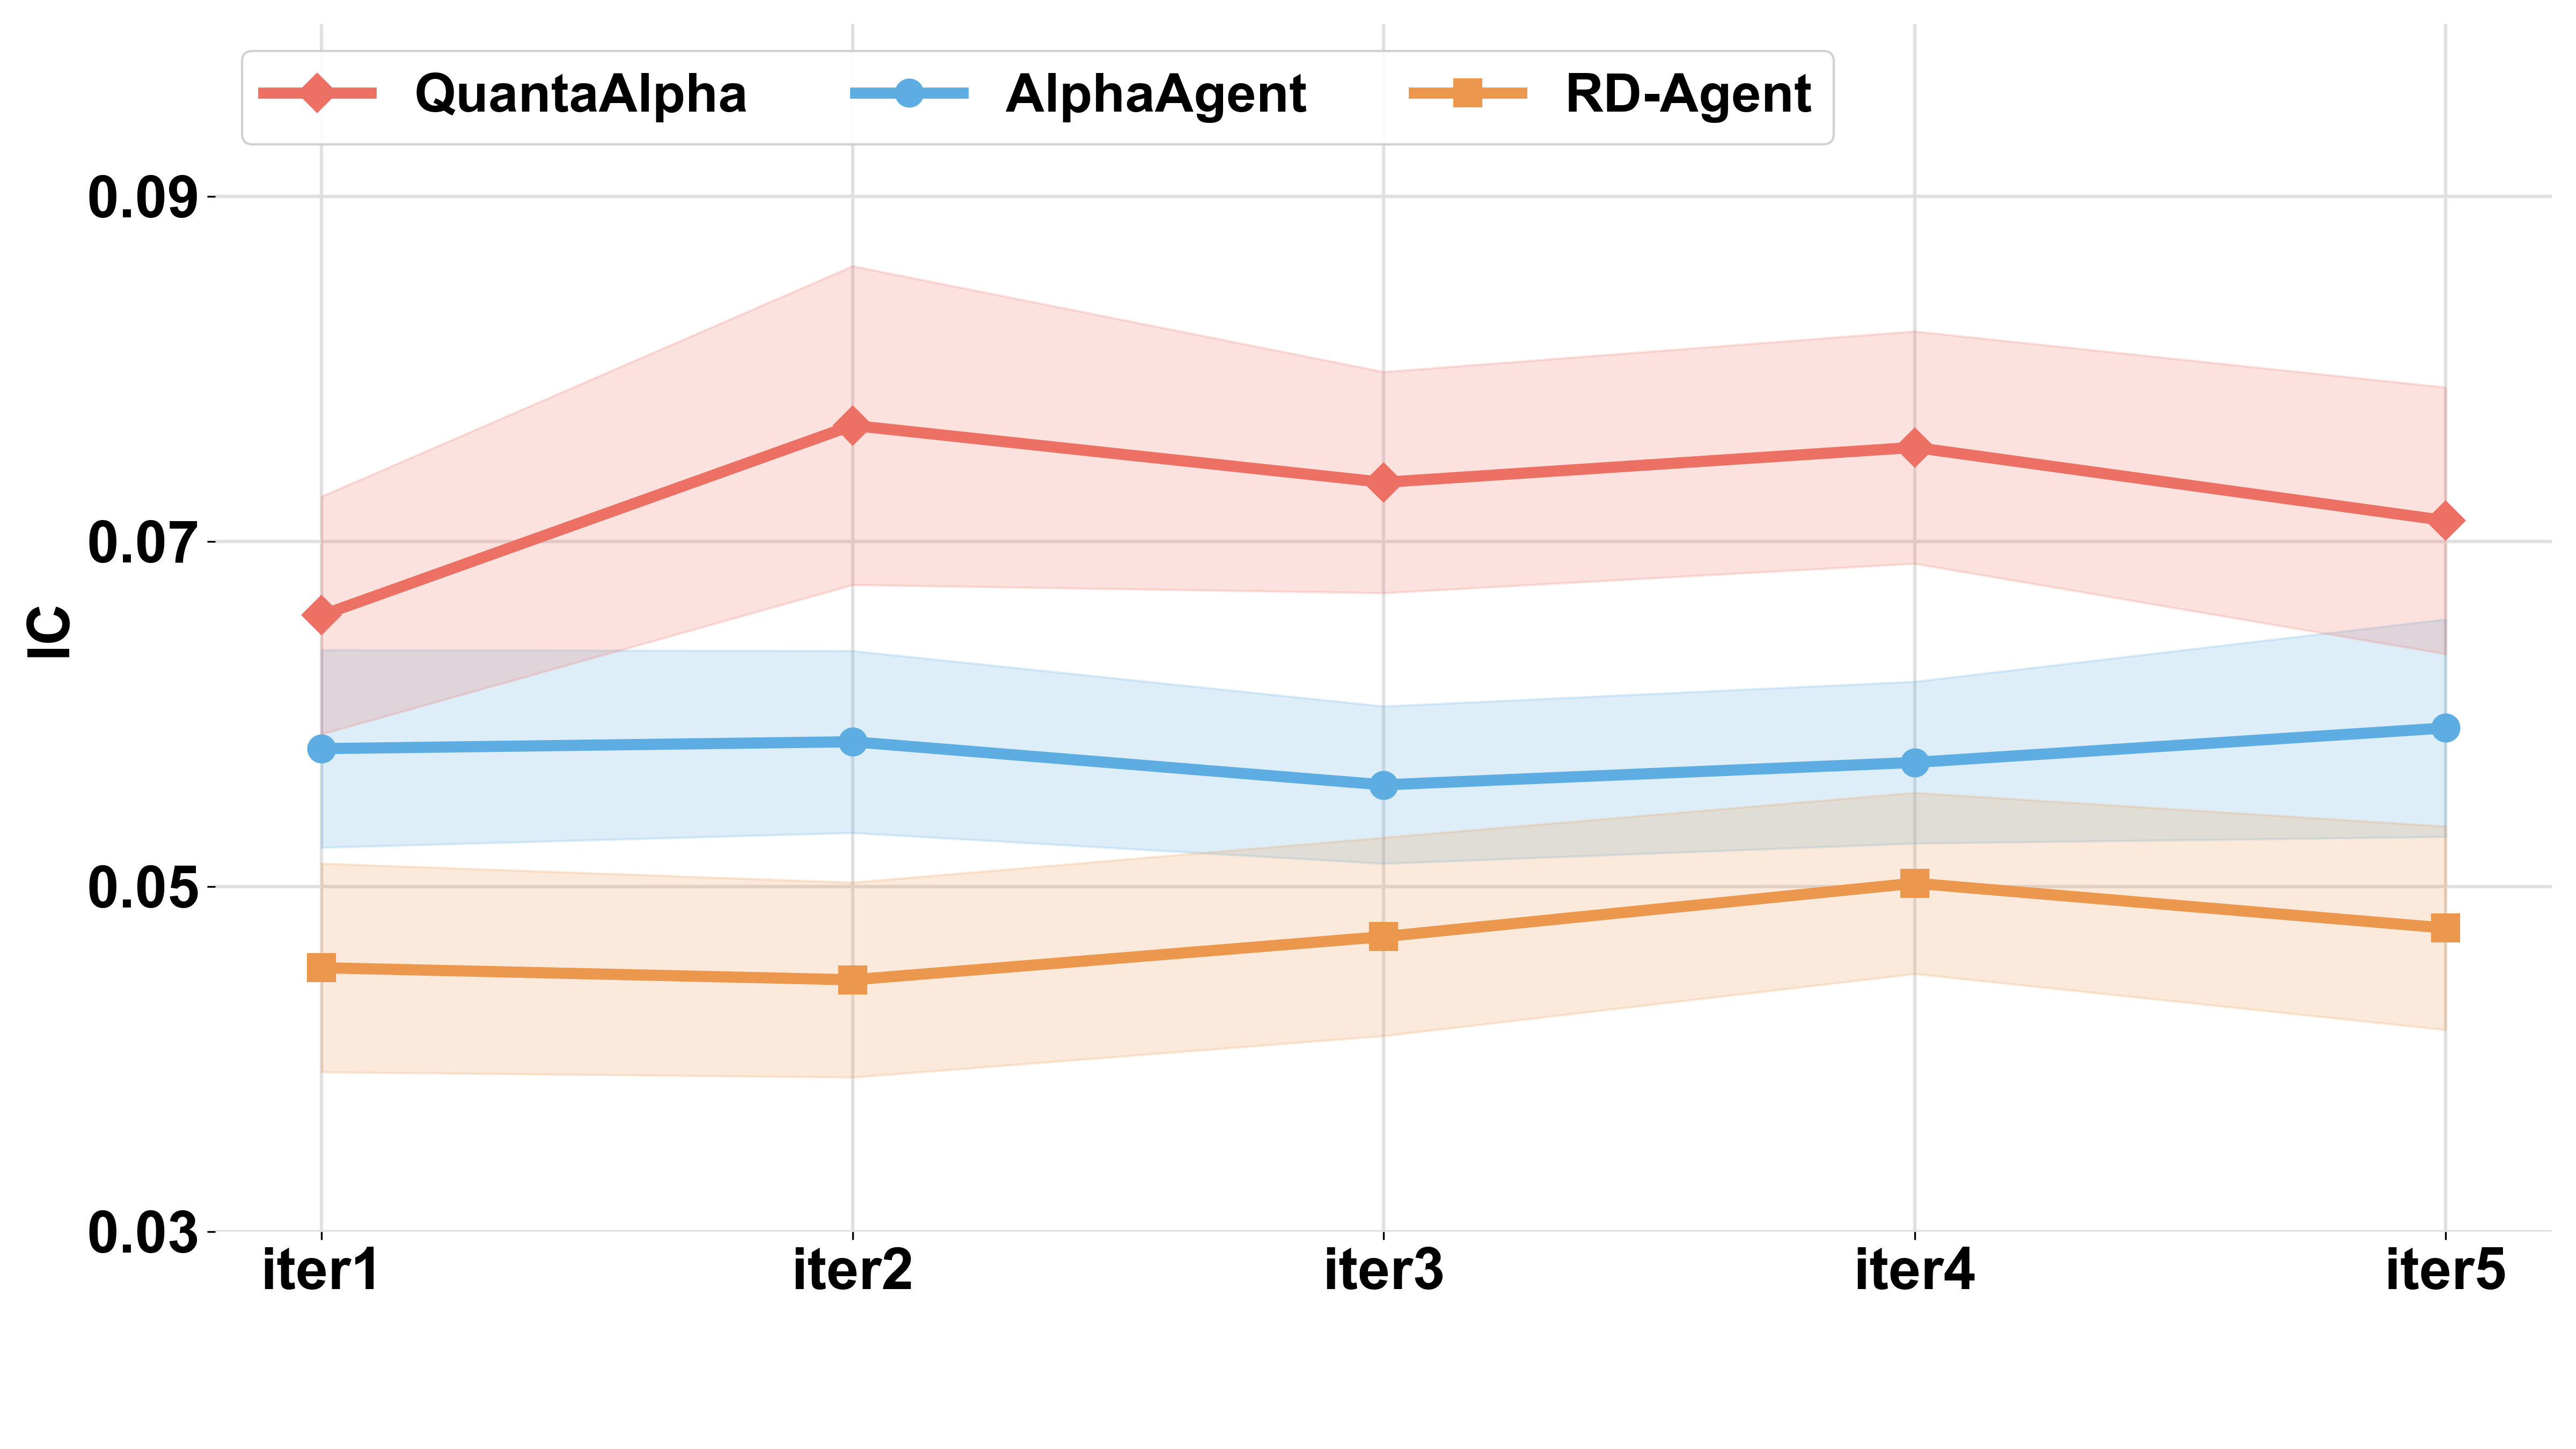
\includegraphics[width=0.6\columnwidth]{images/figu.png}
\caption{The evolution of IC over the first five iterations.}
\label{fig:ic_evolution}
\end{figure}

\subsection{Case Study}
\paragraph{Case Study Setup} To make the evolution process concrete, we present a representative case study and trace how QuantaAlpha updates hypotheses and factors over five iterations. We run QuantaAlpha for a total of 15 iterations on CSI300, using Deepseek-V3.2 as the backbone LLM for all agents. To improve mining throughput, we set the factor-complexity constraints to symbol length $\leq 200$ and base features $\leq 4$. Each iteration consists of two phases: a \textit{Mutation} phase followed by a \textit{Crossover} phase.At the end of each iteration, we maintain a global high-quality factor pool using all factors generated up to that iteration. The maintenance rule is greedy and RankIC-driven: we sort all candidate factors by RankIC (descending) and add them into the pool in order, subject to a redundancy constraint. A factor is admitted only if its absolute correlation with every factor already in the pool is below 0.7. The pool size is capped at 50\% of the total number of mined factors up to the current iteration. 

\begin{figure}[!t]
\centering
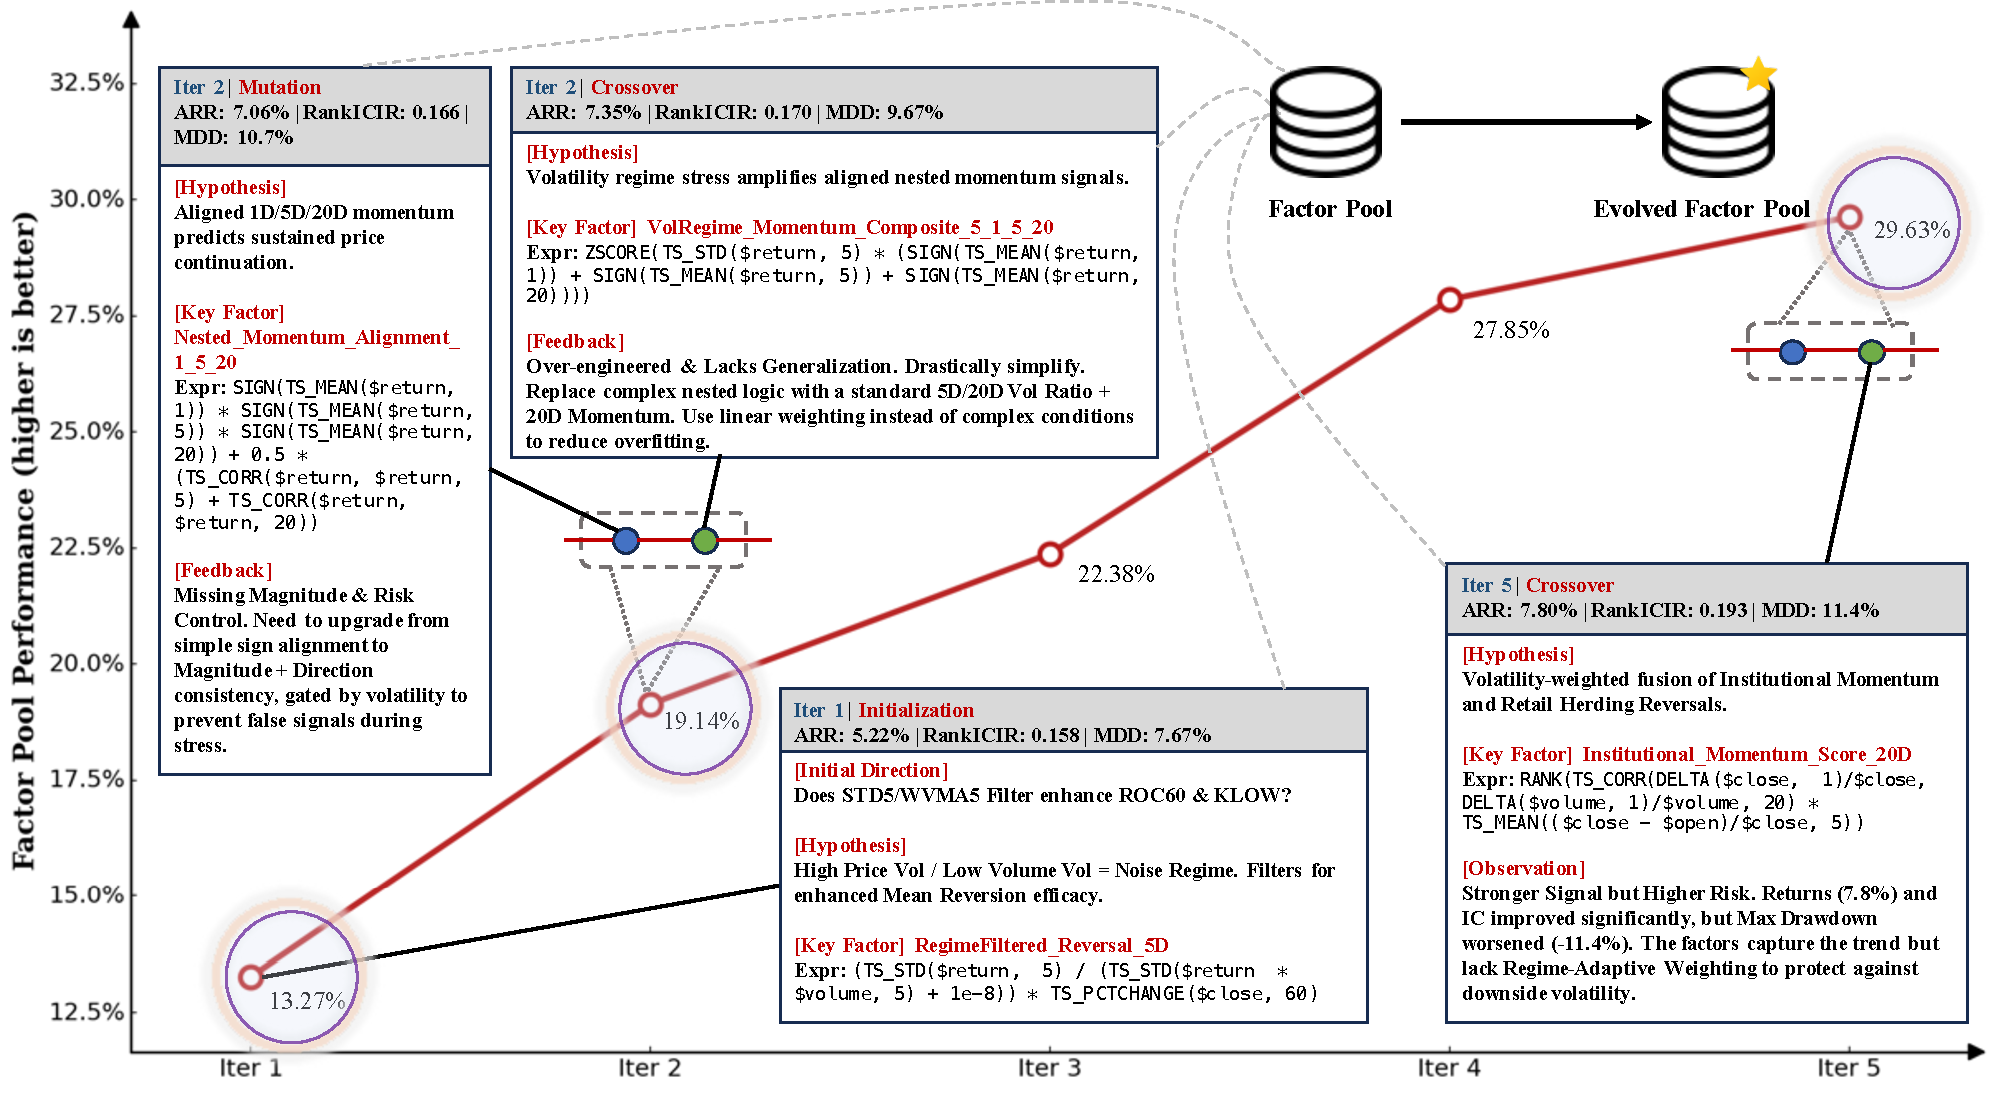
\includegraphics[width=1\textwidth]{images/case_study.pdf}
\caption{A case study of iterative hypothesis and factor updates in QuantaAlpha.}
\label{fig:case_study}
\end{figure}


\paragraph{Factor Example} Figure~\ref{fig:case_study} illustrates how QuantaAlpha refines hypotheses and factor expressions across iterations via the \emph{mutation} and \emph{crossover} phases. The highlighted factors in the figure are therefore representative nodes on different traces across iterations. The first iteration yields interpretable short-term reversal factors. The second broadens the mechanism via volatility-weighted momentum, but increased structural complexity coincides with weaker generalization. Subsequent iterations simplify the expression into a linear additive form, improving drawdown and stabilizing performance. The fifth iteration adds participant-differentiated behavioral signals, incorporating complementary information and further improving predictability. Throughout the evolution, QuantaAlpha maintains a cumulative factor pool. Its predictive performance does not saturate within the first five iterations and only begins to decay after roughly 15 iterations, indicating that the evolution sustains effective improvement over a substantial horizon before diminishing returns emerge.  

\paragraph{Iteration Convergence} Figure~\ref{fig:Iteration_analysis_appendix} illustrates the predictive performance of the factor pool from the fifth iteration onwards. We observe that the predictive performance does not increase linearly with the number of iterations. The strategy's return capacity and risk control ability are gradually optimized, reaching a balanced high level between return and maximum drawdown around the 11th to 12th iterations. Subsequent additional iterations fail to bring significant performance improvement; instead, they may introduce redundant information through newly generated factors, leading to reduced strategy robustness and deteriorated drawdown performance. Overall, the 11th to 12th iterations (approximately 350 factors in total) represent the optimal trade-off point between return level and risk control effect under this experimental setup.


\begingroup
\makeatletter
% If LaTeX decides to put this figure on a float-only page, remove vertical centering.
\setlength{\@fptop}{0pt}
\setlength{\@fpbot}{0pt}
\makeatother
\begin{figure}[!t]
\centering
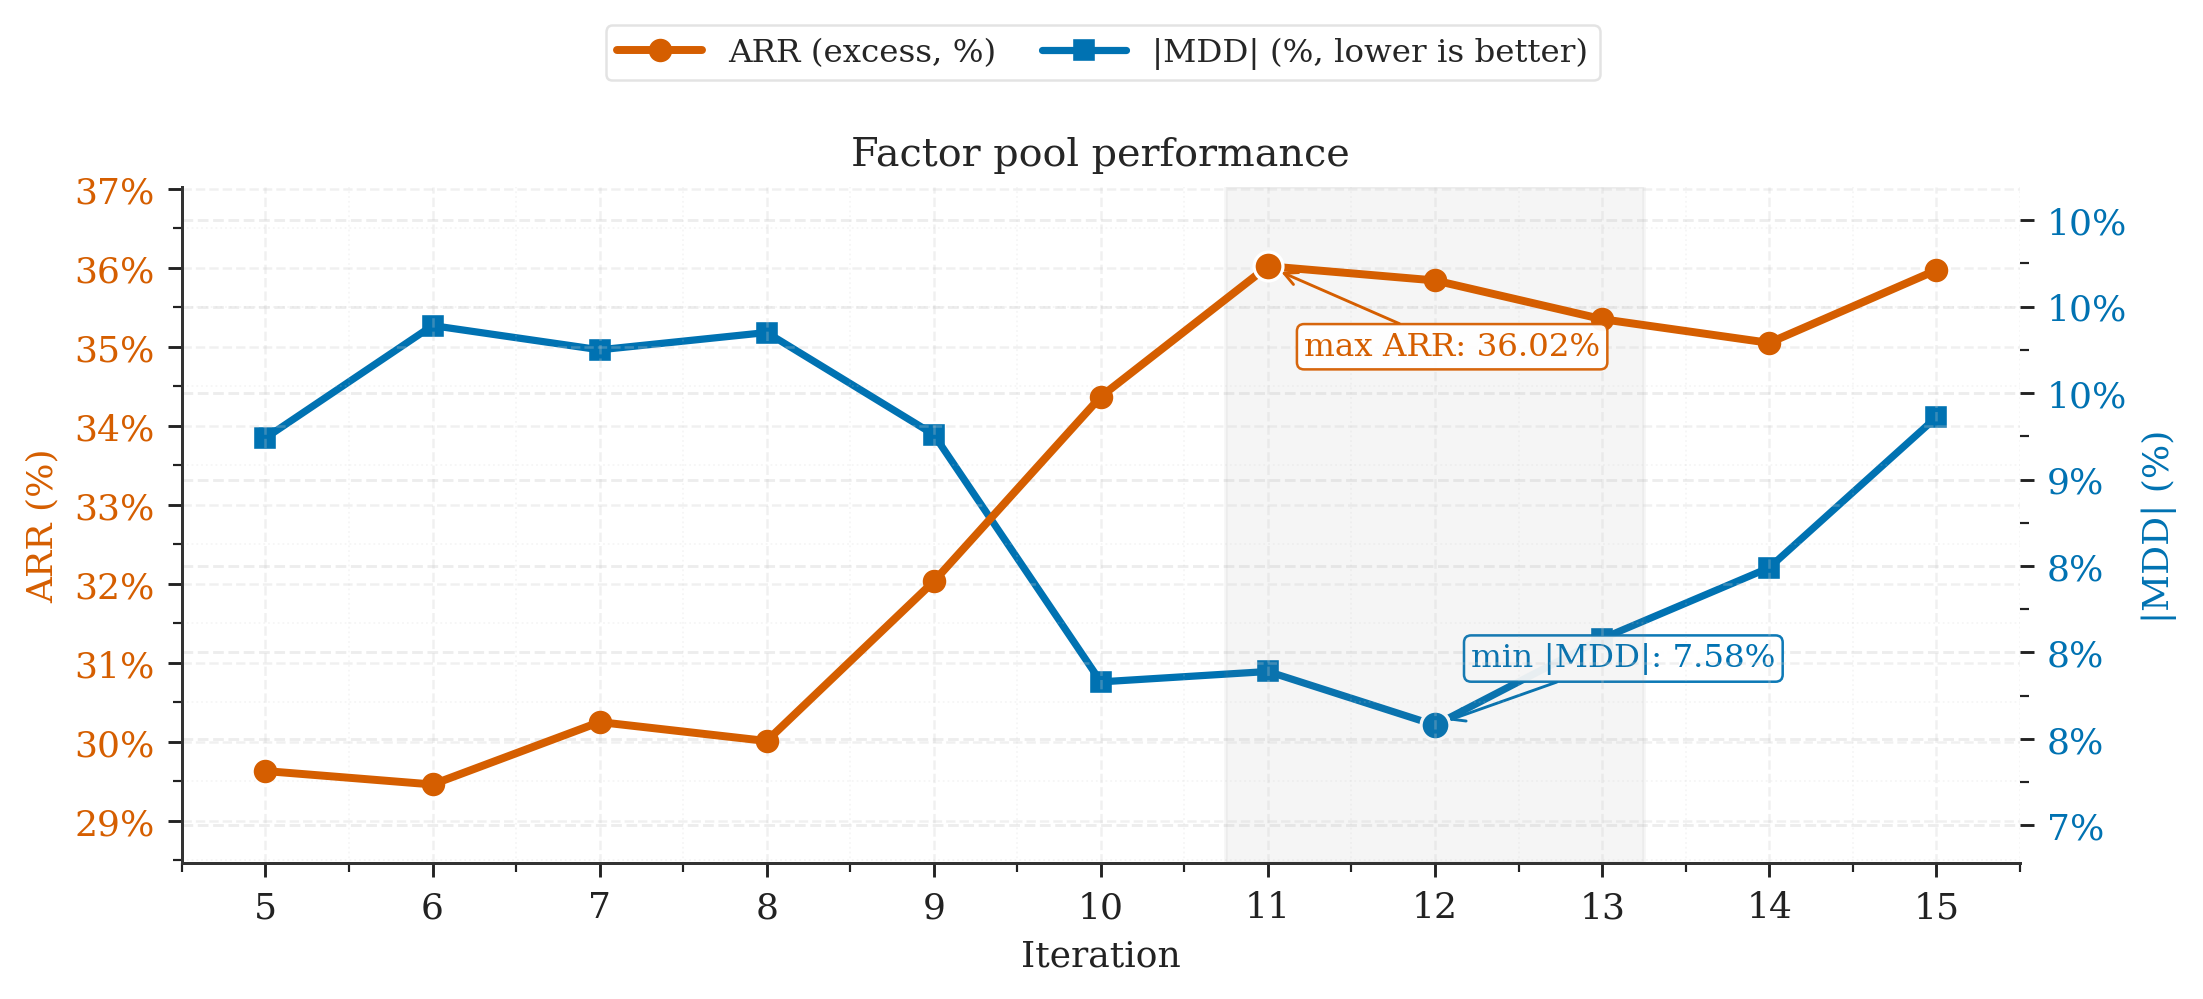
\includegraphics[width=0.95\textwidth]{images/iteration.png}
\caption{Factor Pool Performance by Iteration.}
\label{fig:Iteration_analysis_appendix}
\end{figure}
\endgroup

\section{Conclusion}

We present~\method, a self-evolving framework for interpretable alpha mining that formulates factor discovery as a constrained multi-agent research process. Extensive experiments across both Chinese and U.S. equity markets show that \method consistently produces more stable and generalizable factors than all baselines. Beyond empirical performance, \method emphasizes three properties critical for real-world quantitative research: \emph{diversity}, \emph{controllability}, and \emph{trustworthiness}. Diversity is promoted by broad hypothesis exploration and redundancy-aware evolution, improving robustness under non-stationarity; controllability is enabled by symbolic representations and synthesis-time gates that enforce consistency and limit complexity. Trustworthiness is further strengthened by trajectory-level inheritance, where crossover recombines high-performing segments from previously successful trajectories, providing a verifiable lineage of validated mechanisms and repair patterns. Future work will explore extending \method to multi-asset and cross-market settings, incorporating adaptive regime-aware evolution, and integrating the agentic discovery process more tightly with portfolio construction and risk management. More broadly, we believe that agentic evolution provides a promising paradigm for discovery problems in high-noise, non-stationary domains beyond finance.


\section*{Acknowledgments}
This work was supported by the National Social Science Fund of China Project under Grant No. 22BTJ031; and the Shanghai Engineering Research Center of Finance Intelligence under Grant No. 19DZ2254600. We acknowledge the technical support from the Qinghai Provincial Key Laboratory of Big Data in Finance and Artificial Intelligence Application Technology. 

\bibliography{reference}



\appendix
\onecolumn
\newpage
\centerline{\maketitle{\textbf{SUMMARY OF THE APPENDIX}}}

This appendix contains additional details for the  \textbf{\textit{``QuantaAlpha: An Evolutionary Framework for LLM-Driven Alpha Mining''}}. The appendix is organized as follows:


\startcontents[appendices]
\section*{Appendix Table of Contents}
\printcontents[appendices]{}{0}{\large}



\section{Experiment Settings}
\label{sec:appendix_experiment_details}

This section provides details of our experimental setup, including computational infrastructure, evaluation metrics, backtesting setup, and baselines.

\subsection{Evaluation Metrics}
\label{appendix:A.2}

We evaluate predictive performance using two categories of metrics: factor predictive power and strategy-level performance.

Without loss of generality, the bar notation $\bar{\cdot}$ denotes the mean, and $\sigma(\cdot)$ denotes the standard deviation.

\begin{itemize}
    \setlength{\itemsep}{-2pt}
    \setlength{\parsep}{0pt}
    \setlength{\topsep}{0pt}
    \setlength{\partopsep}{0pt} 
    \item \textbf{Information Coefficient (IC)}: Pearson correlation between factor values $\mathbf{f}_t$ and future returns $\mathbf{r}_{t+1}$:
    \begin{equation*}
        \operatorname{IC}_t = \frac{(\mathbf{f}_t - \bar{f}_t \mathbf{1})^\top (\mathbf{r}_{t+1} - \bar{r}_{t+1} \mathbf{1})}{\|\mathbf{f}_t - \bar{f}_t \mathbf{1}\|_2 \cdot \|\mathbf{r}_{t+1} - \bar{r}_{t+1} \mathbf{1}\|_2},
    \end{equation*}
    where $\mathbf{1}$ denotes a column vector of ones.
    
    \item \textbf{ICIR}: Information ratio of IC, measuring consistency: $\operatorname{ICIR} = \overline{\operatorname{IC}} / \sigma(\operatorname{IC})$.
    
    \item \textbf{Rank IC}: Spearman correlation using rank vectors $\tilde{\mathbf{f}}_t = \operatorname{rank}(\mathbf{f}_t)$ and $\tilde{\mathbf{r}}_{t+1} = \operatorname{rank}(\mathbf{r}_{t+1})$:
    \begin{equation*}
        \operatorname{RankIC}_t = \frac{(\tilde{\mathbf{f}}_t - \bar{\tilde{f}}_t \mathbf{1})^\top (\tilde{\mathbf{r}}_{t+1} - \bar{\tilde{r}}_{t+1} \mathbf{1})}{\|\tilde{\mathbf{f}}_t - \bar{\tilde{f}}_t \mathbf{1}\|_2 \cdot \|\tilde{\mathbf{r}}_{t+1} - \bar{\tilde{r}}_{t+1} \mathbf{1}\|_2},
    \end{equation*}
    where $\operatorname{rank}(\cdot)$ is the rank function applied element-wise to its input vector in ascending order.
    
    \item \textbf{Rank ICIR}: Information ratio of Rank IC: $\operatorname{RankICIR} = \overline{\operatorname{RankIC}} / \sigma(\operatorname{RankIC})$.
\end{itemize}

All strategy metrics are computed on \textit{excess returns after transaction costs}, where $r_{\text{excess},t} = r_{\text{portfolio},t} - r_{\text{benchmark},t} - c_{\text{transaction},t}$. Here, $r_{\text{portfolio},t}$ represents the return of the strategy portfolio, $r_{\text{benchmark},t}$ denotes the return of the market benchmark, and $c_{\text{transaction},t}$ accounts for the transaction costs incurred at time $t$.

\begin{itemize}
    \setlength{\itemsep}{-2pt}
    \setlength{\parsep}{0pt}
    \setlength{\topsep}{0pt}
    \setlength{\partopsep}{0pt}
    \item \textbf{Information Ratio ($\operatorname{IR}$)}: $\operatorname{IR} = (\overline{r_{\text{excess}}} / \sigma(r_{\text{excess}})) \times \sqrt{252}$.
    \item \textbf{Annualized Return ($\operatorname{ARR}$)}: Annualized excess return over benchmark.
    \item \textbf{Maximum Drawdown ($\operatorname{MDD}$)}: Largest peak-to-trough decline in cumulative excess returns.
    \item \textbf{Calmar Ratio ($\operatorname{CR}$)}: $\operatorname{CR} = \operatorname{ARR} / |\operatorname{MDD}|$.
\end{itemize}

\subsection{Backtesting Setup}
\label{subsec:backtest_setup}

Backtesting is conducted using the Qlib framework across the CSI 300, CSI 500, and S\&P 500 indices, with the data split detailed in Table~\ref{tab:data_split}. Factor construction utilizes six basic features—\texttt{open}, \texttt{high}, \texttt{low}, \texttt{close}, \texttt{volume}, and \texttt{vwap}—to predict the next-day return, defined as $y_t = P_{t+2}^{\text{close}} / P_{t+1}^{\text{close}} - 1$, where $P_{t}^{\text{close}}$ denotes the closing price at time $t$. To ensure robustness against outliers, the preprocessing pipeline includes forward-filling missing values, replacing infinite values, dropping samples with missing labels, and applying cross-sectional rank normalization (CSRankNorm) to both features and labels.

\begin{table}[!htbp]
\centering
\caption{Data Split Periods for Train, Validation, and Test Sets across All Markets}
\label{tab:data_split}
\begin{tabular}{lccc}
\toprule
\textbf{Market} & \textbf{Train} & \textbf{Valid} & \textbf{Test} \\
\midrule
CSI 300 & 2016-01-01--2020-12-31 & 2021-01-01--2021-12-31 & 2022-01-01--2025-12-26 \\
CSI 500 & 2016-01-01--2020-12-31 & 2021-01-01--2021-12-31 & 2022-01-01--2025-12-26 \\
S\&P 500 & 2016-01-01--2020-12-31 & 2021-01-01--2021-12-31 & 2022-01-01--2025-12-26 \\
\bottomrule
\end{tabular}
\end{table}

\subsection{Baselines}
\label{appendix:A.5}

We benchmark against four categories: (1) \textbf{ML models}: Linear Regression (Linear), Multi-Layer Perceptron (MLP), and gradient boosting decision trees including LightGBM, XGBoost, and CatBoost, along with DoubleEnsemble, an ensemble method for financial time series; (2) \textbf{Deep learning}: Recurrent networks such as Gated Recurrent Unit (GRU) and Long Short-Term Memory (LSTM), the attention-based Transformer, and Temporal Routing Adaptor (TRA); (3) \textbf{Classical factors}: Alpha158 and Alpha360, which are widely used sets of technical factors derived from price and volume; (4) \textbf{LLM agents}: RD-Agent and AlphaAgent, which utilize large language models for automated factor mining. For the LLM-agent baselines (RD-Agent and AlphaAgent), we evaluate multiple backbone LLMs, including Qwen3-235B, DeepSeek-V3.2, Gemini-3-Pro-Preview, Claude-4.5-Sonnet, and GPT-5.2. Unless otherwise specified, all other LLM-based experiments in this paper adopt DeepSeek-V3.2 for consistency and fair comparison.

\section{Algorithm Configuration}
\label{sec:appendix_algorithm}


This section details the evolution algorithm parameters, factor constraints, and trading strategy configuration.

QuantaAlpha employs an evolutionary algorithm with mutation and crossover operations, with LightGBM used as the downstream model for factor-based prediction. In the Planning Phase of the algorithm, we set ten parallel exploration directions to broaden the initial coverage of research space. For the experimental setup, beyond the original round, the algorithm follows a fixed iterative process: the main experiment consists of 5 total iterations, and each iteration comprises one Mutation phase followed by one Crossover phase—alternating between these two phases to iteratively refine high-quality hypotheses. Additionally, we set a rule that each hypothesis attempts to generate 3 factor expressions, ensuring a focused yet sufficient exploration of factor candidates under each research direction.

To prevent overfitting and ensure interpretability, factor expressions—built using the operators listed in Table~\ref{tab:factor_operators}—are restricted by the following constraints: symbol length $\le$ 250 characters, base features $\le$ 6, free arguments ratio $<$ 50%, and duplicate subtree size $\le$ 5. Details of the associated complexity penalty formulation are discussed in the main text.

\begin{table}[!htbp]
\centering
\caption{List of Supported Operators for Factor Construction}
\label{tab:factor_operators}
\small
\setlength{\tabcolsep}{4pt}
\begin{tabular}{p{2.3cm} p{8cm} @{\hspace{0.6cm}} p{5.5cm}}
\toprule
\textbf{Category} & \textbf{Operators} & \textbf{Description} \\
\midrule
Time-Series & \texttt{DELTA}, \texttt{DELAY}, \texttt{TS\_MEAN}, \texttt{TS\_STD}, \texttt{TS\_VAR}, \texttt{TS\_MAX}, \texttt{TS\_MIN}, \texttt{TS\_SUM}, \texttt{TS\_RANK}, \texttt{TS\_CORR}, \texttt{TS\_COVARIANCE}, \texttt{TS\_ARGMAX}, \texttt{TS\_ARGMIN}, \texttt{TS\_SKEW}, \texttt{TS\_KURT}, \texttt{TS\_PCTCHANGE}, \texttt{TS\_ZSCORE}, \texttt{TS\_QUANTILE} & Rolling statistics computed along time axis per instrument \\
\midrule
Cross-Sectional & \texttt{RANK}, \texttt{ZSCORE}, \texttt{SCALE}, \texttt{MEAN}, \texttt{STD}, \texttt{MEDIAN}, \texttt{MAX}, \texttt{MIN}, \texttt{SKEW}, \texttt{KURT} & Statistics computed across stocks per datetime \\
\midrule
Mathematical & \texttt{ABS}, \texttt{SIGN}, \texttt{LOG}, \texttt{EXP}, \texttt{SQRT}, \texttt{POW}, \texttt{INV} & Element-wise mathematical functions \\
\midrule
Technical & \texttt{SMA}, \texttt{EMA}, \texttt{WMA}, \texttt{MACD}, \texttt{RSI}, \texttt{BB\_UPPER}, \texttt{BB\_LOWER}, \texttt{DECAYLINEAR}, \texttt{REGBETA}, \texttt{REGRESI} & Common technical indicators \\
\midrule
Logical & \texttt{GT}, \texttt{LT}, \texttt{GE}, \texttt{LE}, \texttt{AND}, \texttt{OR}, \texttt{WHERE} & Comparison and conditional operators \\
\midrule
Auxiliary & \texttt{COUNT}, \texttt{SUMIF}, \texttt{FILTER}, \texttt{PROD}, \texttt{HIGHDAY}, \texttt{LOWDAY} & Helper functions for complex expressions \\
\bottomrule
\end{tabular}
\end{table}


We employ a TopkDropout strategy for portfolio construction, as detailed in Table~\ref{tab:trading_params}. On each trading day, stocks are ranked according to their predicted scores; the $n_{\text{drop}}$ lowest-scoring holdings are liquidated and replaced with the highest-ranked candidates to maintain a constant portfolio size with equal weighting.

\begin{table}[!htbp]
\centering
\caption{Parameters for the TopkDropout Trading Strategy}
\label{tab:trading_params}
\begin{tabular}{llp{5cm}}
\toprule
\textbf{Parameter} & \textbf{Value} & \textbf{Description} \\
\midrule
\multicolumn{3}{c}{\textit{Portfolio}} \\
\midrule
topk & 50 & Number of stocks held \\
n\_drop & 5 & Stocks dropped per rebalance \\
\midrule
\multicolumn{3}{c}{\textit{Transaction Costs}} \\
\midrule
Buying Fee & 0.05\% & Commission \\
Selling Fee & 0.15\% & Commission + stamp duty \\
\midrule
\multicolumn{3}{c}{\textit{Execution}} \\
\midrule
Deal Price & Open & Next-day opening price \\
Limit Threshold & 9.5\% & Price limit for halt \\
\midrule
\multicolumn{3}{c}{\textit{Benchmark}} \\
\midrule
China & SH000300/SH000905 & CSI 300/CSI500 \\
U.S. & SPX & S\&P 500 \\
\bottomrule
\end{tabular}
\end{table}
%%%%%%%%%%%%%%%%%%%%%%%%%%%%%%%%%%%%%%%%%%%%%%%%%%%%%%%%%%%%%%%%%%%%%%%
% NOTE: Add the following to your main document preamble:
%
% \usepackage{xcolor}
% \usepackage{tcolorbox}
% \tcbuselibrary{skins,breakable}
% \usepackage{tikz}
% \usepackage{fontawesome5}
% \usepackage{booktabs}
%
\definecolor{headerblue}{RGB}{41, 128, 185}
\definecolor{metricgreen}{RGB}{39, 174, 96}
\definecolor{alertred}{RGB}{192, 57, 43}
\definecolor{warningyellow}{RGB}{243, 156, 18}
\definecolor{lightblue}{RGB}{240, 245, 255}
\definecolor{darkblue}{RGB}{30, 60, 120}
\definecolor{mutationpurple}{RGB}{142, 68, 173}
\definecolor{crossoverblue}{RGB}{52, 152, 219}
%
%%%%%%%%%%%%%%%%%%%%%%%%%%%%%%%%%%%%%%%%%%%%%%%%%%%%%%%%%%%%%%%%%%%%%%%

\section{Case Study: Factor Evolution Trajectory}
\label{sec:appendix_case_study}

This appendix presents a detailed case study of factor evolution in QuantaAlpha. We trace the complete trajectory of a representative factor---\textit{Institutional\_Momentum\_Score\_20D}---through the crossover phase, demonstrating how the evolutionary framework synthesizes complementary market hypotheses from parent trajectories.

QuantaAlpha's evolution process operates in three phases: (1) \textbf{Original} phase where initial hypotheses are generated, (2) \textbf{Mutation} phase where existing trajectories are perturbed to explore diversified strategies, and (3) \textbf{Crossover} phase where high-performing parent trajectories are combined to synthesize offspring with potentially superior predictive power. The following factor card illustrates a Crossover operation.

%%%%%%%%%%%%%%%%%%%%%%%%%%%%%%%%%%%%%%%%%%%%%%%%%%%%%%%%%%%%%%%%%%%%%%%
% Factor Identity Card
%%%%%%%%%%%%%%%%%%%%%%%%%%%%%%%%%%%%%%%%%%%%%%%%%%%%%%%%%%%%%%%%%%%%%%%
\subsection{Factor Identity}

The factor card below presents the basic information of the evolved factor, including its unique identifiers, evolution lineage, and mathematical formulation.

\begin{tcolorbox}[
  colback=lightblue,
  colframe=darkblue,
  fonttitle=\bfseries,
  title={\faTag\ Institutional\_Momentum\_Score\_20D},
  arc=2mm,
  boxrule=0.5pt,
  breakable
]

\begin{tabular}{@{}ll@{}}
\textbf{Factor ID:} & \texttt{c57cace576a95356} \\
\textbf{Trajectory ID:} & \texttt{df5a496878f4} \\
\textbf{Evolution Round:} & Round 10 \\
\textbf{Evolution Phase:} & \colorbox{crossoverblue!20}{\textcolor{crossoverblue}{\textbf{Crossover}}} \\
\textbf{Direction ID:} & 6 \\
\end{tabular}

\vspace{0.3cm}

\textbf{Factor Expression:}
\begin{tcolorbox}[colback=darkblue!5, colframe=darkblue, boxrule=0.3pt, arc=1mm]
\small\ttfamily
RANK(TS\_CORR(DELTA(close, 1)/close, DELTA(volume, 1)/volume, 20) * TS\_MEAN((close - open)/close, 5))
\end{tcolorbox}

\textbf{Mathematical Formulation:}
\[
\text{IMS}_{20D} = \text{RANK}\left(\rho_{20}\left(\frac{\Delta P}{P}, \frac{\Delta V}{V}\right) \times \overline{\left(\frac{C - O}{C}\right)}_{5}\right),
\]
\small
where $\rho_{20}(\cdot,\cdot)$ denotes the 20-day rolling correlation, $\Delta P/P$ is the daily return, $\Delta V/V$ is the volume change ratio, $\overline{(\cdot)}_5$ is the 5-day moving average, and $C$ and $O$ represent the closing and opening prices, respectively.

\vspace{0.2cm}

\textbf{Factor Interpretation:}\\
\small
This factor captures institutional-driven momentum by measuring two key signals: (1) the correlation between price returns and volume changes, which indicates coordinated institutional trading when positive; and (2) the average intraday return pattern, reflecting institutional activity that typically influences closing prices. The cross-sectional ranking ensures comparability across stocks.

\end{tcolorbox}

%%%%%%%%%%%%%%%%%%%%%%%%%%%%%%%%%%%%%%%%%%%%%%%%%%%%%%%%%%%%%%%%%%%%%%%
% Evolution Lineage
%%%%%%%%%%%%%%%%%%%%%%%%%%%%%%%%%%%%%%%%%%%%%%%%%%%%%%%%%%%%%%%%%%%%%%%
\subsection{Evolution Lineage}

The crossover operation combines insights from two parent trajectories with complementary market hypotheses. Parent 1 focuses on identifying \textit{fragile momentum} driven by retail speculation, while Parent 2 targets \textit{sustainable momentum} supported by institutional activity. The LLM synthesizes these complementary perspectives into a unified framework.

\begin{tcolorbox}[
  colback=lightblue,
  colframe=darkblue,
  fonttitle=\bfseries,
  title={\faDna\ Evolution Information},
  arc=2mm,
  boxrule=0.5pt,
  breakable
]

\textbf{\faCodeBranch\ Parent Trajectories:}

\vspace{0.3cm}

\begin{tcolorbox}[colback=lightblue, colframe=darkblue!50, boxrule=0.3pt, title={\small\textbf{Parent 1: 1e6d57e38e89}}, fonttitle=\bfseries\small]
\small
\begin{tabular}{@{}ll@{}}
\textbf{Round:} & Round 9 \\
\textbf{Phase:} & Mutation \\
\textbf{Rank IC:} & 0.0216 \\
\textbf{IC:} & 0.0059 \\
\textbf{IR:} & 1.297 \\
\end{tabular}

\vspace{0.2cm}
\textbf{Core Hypothesis:}\\
\small
When retail investors exhibit herd behavior and momentum chasing in stocks with high social media activity, but accompanied by declining institutional ownership and deteriorating fundamentals, the resulting price momentum is unsustainable and leads to mean reversion.
\end{tcolorbox}

\vspace{0.2cm}

\begin{tcolorbox}[colback=lightblue, colframe=darkblue!50, boxrule=0.3pt, title={\small\textbf{Parent 2: 47e0f0e55382}}, fonttitle=\bfseries\small]
\small
\begin{tabular}{@{}ll@{}}
\textbf{Round:} & Round 8 \\
\textbf{Phase:} & Crossover \\
\textbf{Rank IC:} & 0.0246 \\
\textbf{IC:} & 0.0069 \\
\textbf{IR:} & 1.347 \\
\end{tabular}

\vspace{0.2cm}
\textbf{Core Hypothesis:}\\
\small
A regime-adaptive structural momentum factor combining institutional ownership-driven medium-term price trends with short-term microstructure regime validation, where coordinated accumulation/distribution patterns amplify momentum when confirmed by microstructure alignment.
\end{tcolorbox}

\vspace{0.3cm}

\textbf{\faSitemap\ Evolution Path Diagram:}
\begin{center}
\resizebox{0.7\linewidth}{!}{%
\begin{tikzpicture}[
    node distance=1.5cm,
    roundbox/.style={rectangle, rounded corners, align=center, font=\scriptsize},
    parentbox/.style={roundbox, draw=darkblue!60, fill=lightblue, minimum width=2.5cm, minimum height=0.8cm},
    childbox/.style={roundbox, draw=darkblue, fill=darkblue!15, minimum width=3cm},
    arrow/.style={->, thick, >=stealth, color=darkblue}
]
    % Parent nodes
    \node[parentbox] (p1) at (-2.5, 1.8) {Parent 1\\Round 9 Mutation\\Rank IC: 0.0216};
    \node[parentbox] (p2) at (2.5, 1.8) {Parent 2\\Round 8 Crossover\\Rank IC: 0.0246};
    
    % Current node
    \node[childbox] (current) at (0, 0) {\textbf{Offspring Factor}\\Round 8 Crossover\\Rank IC: \textbf{0.0311}};
    
    % Arrows
    \draw[arrow] (p1) -- (current);
    \draw[arrow] (p2) -- (current);
    
    % Label
\end{tikzpicture}%
}
\end{center}

\end{tcolorbox}

%%%%%%%%%%%%%%%%%%%%%%%%%%%%%%%%%%%%%%%%%%%%%%%%%%%%%%%%%%%%%%%%%%%%%%%
% Synthesized Hypothesis
%%%%%%%%%%%%%%%%%%%%%%%%%%%%%%%%%%%%%%%%%%%%%%%%%%%%%%%%%%%%%%%%%%%%%%%
\subsection{Synthesized Hypothesis}

Through crossover, the LLM generates a new hypothesis that integrates the complementary insights from both parents, rather than simply averaging their factor expressions. This hypothesis-driven approach ensures that the offspring factor captures genuinely novel market dynamics.

\begin{tcolorbox}[
  colback=lightblue,
  colframe=darkblue,
  fonttitle=\bfseries,
  title={\faLightbulb\ Hypothesis},
  arc=2mm,
  boxrule=0.5pt,
  breakable
]

\textbf{Core Hypothesis:}\\
A regime-aware dual-source momentum factor that combines institutional-driven structural momentum (validated by healthy microstructure) and retail-driven speculative momentum (characterized by high attention and deteriorating fundamentals), dynamically weighted by market volatility: amplifying institutional signals in stable regimes and retail reversal signals in turbulent regimes, will generate superior predictive returns.

\vspace{0.3cm}

\begin{tabular}{@{}p{0.28\textwidth}p{0.67\textwidth}@{}}
\toprule
\textbf{Component} & \textbf{Description} \\
\midrule
\textbf{Observation} & Parent strategies separately targeting institutional trends and retail herding show moderate predictive power (Rank IC $\sim$0.02--0.025), suggesting combined signals could capture complementary market dynamics. \\
\midrule
\textbf{Justification} & Sustainable price trends require institutional sponsorship and orderly trading, while retail-driven bubbles lack fundamental support and reverse under stress; a hybrid model exploiting both can enhance robustness across market regimes. \\
\midrule
\textbf{Domain Knowledge} & Institutional accumulation with strong price-volume correlation and low volatility indicates sustainable momentum; retail herding with declining institutional ownership and high volatility signals fragile momentum prone to reversal. \\
\bottomrule
\end{tabular}

\end{tcolorbox}

%%%%%%%%%%%%%%%%%%%%%%%%%%%%%%%%%%%%%%%%%%%%%%%%%%%%%%%%%%%%%%%%%%%%%%%
% Backtest Results
%%%%%%%%%%%%%%%%%%%%%%%%%%%%%%%%%%%%%%%%%%%%%%%%%%%%%%%%%%%%%%%%%%%%%%%
\subsection{Backtest Performance}

After factor construction, QuantaAlpha automatically backtests the generated factors using the Qlib framework. The results below compare the offspring factor against both parent trajectories and the baseline, demonstrating the effectiveness of the crossover operation.

\begin{tcolorbox}[
  colback=lightblue,
  colframe=darkblue,
  fonttitle=\bfseries,
  title={\faChartLine\ Backtest Metrics},
  arc=2mm,
  boxrule=0.5pt,
  breakable
]

\begin{center}
\begin{tabular}{@{}lccc@{}}
\toprule
\textbf{Metric} & \textbf{Offspring Factor} & \textbf{Baseline} \\
\midrule
\textbf{IC} & 0.0126 & 0.0058 \\
\textbf{Rank IC} & \textbf{0.0311} & 0.0220 \\
\midrule
\textbf{ARR (Excess)} & 7.80\% & 5.20\% \\
\textbf{IR} & 0.963 & 0.973 \\
\textbf{MDD (Excess)} & $-$11.37\% & $-$7.30\% \\
\bottomrule
\end{tabular}
\end{center}

\vspace{0.3cm}

\textbf{Detailed Statistics:}
\begin{center}
\small
\begin{tabular}{@{}ll|ll@{}}
\toprule
\textbf{Metric} & \textbf{Value} & \textbf{Metric} & \textbf{Value} \\
\midrule
\textbf{Daily Excess Return (w/o cost)} & 0.0328\% & \textbf{Daily Excess Return (w/ cost)} & 0.0128\% \\
\textbf{Excess Return Std} & 0.52\% & \textbf{Turnover (FFR)} & 100\% \\
\textbf{L2 Train Loss} & 0.9936 & \textbf{L2 Valid Loss} & 0.9962 \\
\bottomrule
\end{tabular}
\end{center}

\end{tcolorbox}

%%%%%%%%%%%%%%%%%%%%%%%%%%%%%%%%%%%%%%%%%%%%%%%%%%%%%%%%%%%%%%%%%%%%%%%
% LLM Summary
%%%%%%%%%%%%%%%%%%%%%%%%%%%%%%%%%%%%%%%%%%%%%%%%%%%%%%%%%%%%%%%%%%%%%%%
\subsection{Trajectory Summary}

After evaluating backtest results, the LLM provides structured summary. This trajectory summary loop enables continuous improvement by learning from both successes and failures.

\begin{tcolorbox}[
  colback=lightblue,
  colframe=darkblue,
  fonttitle=\bfseries,
  title={\faComments\ Evaluation \& Summary},
  arc=2mm,
  boxrule=0.5pt,
  breakable
]

\textbf{\faSearch\ Observations:}\\
The crossover operation demonstrates a trade-off between enhanced predictive accuracy and increased risk exposure compared to the baseline:
\begin{itemize}
    \item \textcolor{metricgreen}{\faCheckCircle} Significant improvement in annualized excess return and predictive metrics (IC and Rank IC), validating the effectiveness of synthesizing dual-source momentum signals.
    \item \textcolor{alertred}{\faTimesCircle} Increased maximum drawdown and a marginal decline in the Information Ratio, suggesting that the offspring factor introduces higher volatility during certain market regimes.
\end{itemize}

\vspace{0.2cm}

\textbf{\faBalanceScale\ Hypothesis Evaluation:}\\[0.15cm]
\small
Results partially support the hypothesis. Improved annualized return and IC suggest that combining institutional and retail momentum signals has merit. However, deterioration in risk metrics indicates that without proper regime-adaptive weighting, the combined signals may amplify risks during turbulent periods. The full hypothesis requires all three components (institutional momentum, retail herding reversal, volatility-adaptive weighting) to work effectively.

\vspace{0.2cm}

\textbf{\faFlag\ Decision:} \colorbox{alertred!20}{\textcolor{alertred}{\textbf{REJECTED}}} for direct deployment.

\vspace{0.2cm}

\textbf{\faExclamationTriangle\ Recommendations:}
\begin{enumerate}
    \setlength{\itemsep}{0pt}
    \setlength{\parsep}{0pt}
    \setlength{\topsep}{0pt}
    \setlength{\partopsep}{0pt}
    \small
    \item Use 20-day price-volume correlation as institutional momentum proxy;
    \item Use 5-day average intraday returns as retail attention proxy;
    \item Add volatility regime indicator (recent/historical volatility ratio) for dynamic weighting.
\end{enumerate}

\small This summary will inform the next mutation round, guiding the LLM to simplify the factor expression while preserving the core dual-source concept.

\end{tcolorbox}

%%%%%%%%%%%%%%%%%%%%%%%%%%%%%%%%%%%%%%%%%%%%%%%%%%%%%%%%%%%%%%%%%%%%%%%%%%%%%%
%%%%%%%%%%%%%%%%%%%%%%%%%%%%%%%%%%%%%%%%%%%%%%%%%%%%%%%%%%%%%%%%%%%%%%%%%%%%%%

\end{document}
